% Autor = dyfmeks
% Date = 20/05/2024

% Preamble
\documentclass[stu, 12pt, letterpaper, donotrepeattitle, floatsintext, natbib]{apa7}
\setlength{\headheight}{15.35403pt}

% Packages
\usepackage[utf8]{inputenc}
\usepackage{comment}
\usepackage{marvosym}
\usepackage{graphicx}
\usepackage{float}
\usepackage[normalem]{ulem}
\usepackage[spanish]{babel}
\usepackage{apacite}
\usepackage{tabularx}
\usepackage{longtable}
% \usepackage[style=apa,sortcites=true,sorting=nyt,backend=biber]{biblatex}
\usepackage{standalone}
\usepackage{csquotes}
\usepackage[page]{appendix}
\usepackage{listings}
\usepackage{subcaption}
\selectlanguage{spanish}
\useunder{\uline}{\ul}{}
\newcommand{\myparagraph}[1]{\paragraph{#1}\mbox{}\\}
%\usepackage[section]{placeins}
%\usepackage{csquotes}
%\usepackage{array,fancyvrb,graphicx,verbatim,xurl}

% Config
%\DeclareLanguageMapping{american}{american-apa}
% \addbibresource{bibliography.bib}
\thispagestyle{empty}
\title{OPTIMIZACI\'ON DE LA GESTI\'ON DE INVENTARIO DE EQUIPOS MEDIANTE EL DISE\~{N}O E IMPLEMENTACI\'ON DE UN MODULO CON GESTI\'ON DE MOVIMIENTOS Y REPORTES}
\shorttitle{Gesti\'on de Inventario de Equipos}
\author{John Jordan Quispe Supo}
\authorsaffiliations{Instituto de Educaci\'on Superior Privado del Sur}
\course{Desarrollo de Sistemas de Informaci\'on}
\professor{Gustavo Delgado Ugarte}
\duedate{20/05/2024}

%\abstract{Este proyecto se centra en el dise\~{n}o y desarrollo de un Sistema de Informaci\'on Integral para la Gesti\'on de
%Conquistadores, Actividades y Progresos en el Club de Conquistadores. El sistema propuesto permitir\'a el registro de
%nuevos conquistadores, la planificaci\'on y registro de actividades, el seguimiento del avance de los conquistadores en
%sus especialidades y clases, y la toma de asistencia y actividades semanales en la unidad. Este trabajo busca optimizar
%la gesti\'on del club, mejorar la eficiencia de las actividades y proporcionar una plataforma web para el seguimiento y
%desarrollo de los conquistadores. Se espera que este sistema integral mejore significativamente la administraci\'on del
%club y enriquezca la experciencia de los conquistadores.}
%\keywords{Sistema de Informaci\'on Integral, Gesti\'on de Conquistadores, Registro de Actividades, Seguimiento de Progresos,
%Club de Conquistadores, Planificaci\'on de Actividades, Toma de Asistencia, Actividades Semanales, Especialidades y Clases
%de Conquistadores, Plataforma Web, Optimizaci\'on de la Gesti\'on, Eficiencia de las Actividades}

% Document
\begin{document}
\maketitle
% \renewcommand\bibname{Bibliografia}
\renewcommand\refname{\textbf{Bibliograf\'{\i}a}}
%   Indices
\pagenumbering{roman}
%   Contenido
\renewcommand\contentsname{\'Indice}
\tableofcontents
\setcounter{tocdepth}{2}
\newpage
%   Figuras
\renewcommand\listfigurename{\'Indice de Figuras}
\listoffigures
\newpage
%   Tablas
\renewcommand\listtablename{\'Indice de Tablas}
\listoftables
\newpage
\renewcommand\lstlistlistingname{\'Indice de C\'odigos}
\renewcommand\lstlistingname{C\'odigo}
\lstlistoflistings\newpage

%   Cuerpo
\pagenumbering{arabic}

% \section{T\'ITULO}
% \noindent OPTIMIZACI\'ON DE LA GESTI\'ON DE INVENTARIO DE EQUIPOS MEDIANTE EL DISE\~{N}O E IMPLEMENTACI\'ON DE UN MODULO CON GESTI\'ON DE MOVIMIENTOS Y REPORTES

% \section{DATOS DEL AUTOR}
% \begin{tabular}{@{} p{2cm} p{12.8cm} @{}}
%     \textbf{Nombres}   & : John Jordan                                                                                            \\
%     \textbf{Apellidos} & : Quispe Supo                                                                                            \\
%     \textbf{Carrera}   & : Desarrollo de Sistemas de Informaci\'on                                                                \\
%     \textbf{Rese\~{n}a}    & : Soy egresado del Instituto del Sur y actualmente laboro en Soluciones de Informaci\'on NextSoft S.A.C. \\
% \end{tabular}
% \newline

% \section{RESUMEN}
% El presente proyecto se centra en el desarrollo de un m\'odulo de gesti\'on de inventario de equipos, dise\~{n}ado para optimizar el control de recursos en una organizaci\'on. Este m\'odulo permite el registro
% detallado de equipos, la gesti\'on de movimientos (entregas a responsables, devoluciones a almac\'en) y las transferencias entre almacenes. Adem\'as, incluye funcionalidades para el mantenimiento de datos
% maestros como marcas, modelos, productos y categor\'{\i}as. El sistema tambi\'en genera reportes exhaustivos que facilitan la toma de decisiones, mejorando la eficiencia en la administraci\'on de los equipos.
% La implementaci\'on del m\'odulo fue realizada utilizando tecnolog\'{\i}as actuales, asegurando su integrabilidad y escalabilidad dentro de la infraestructura existente de la organizaci\'on.


\section{Introducci\'on}
\subsection{Contexto y Antecedentes}
\subsubsection{Descripci\'on de la Unidad de Estudio}
% \begin{tabular}{@{} p{4.3cm} p{9.5cm} @{}}
%     \textbf{RUC}                   & : 20454819137                                                                                                                                         \\
%     \textbf{Raz\'on Social}        & : Soluciones de Informaci\'on NextSoft S.A.C.                                                                                                         \\
%     \textbf{Inicio de Actividades} & : 01/05/2008                                                                                                                                          \\
%     \textbf{Actividad principal}   & : Brinda soluciones inform\'aticas a trav\'es de un sistema ERP personalizado y desarrollos a medida para empresas locales, nacionales e internacionales.
% \end{tabular}
El presente proyecto se llevar\'a a cabo en Soluciones de Informaci\'on NextSoft S.A.C. con RUC 20454819137, una empresa especializada en el desarrollo de soluciones tecnol\'ogicas para la gesti\'on empresarial.
Fundada con el objetivo de ofrecer servicios de alta calidad en el \'ambito de la tecnolog\'{\i}a de la informaci\'on, NextSoft S.A.C. se ha consolidado como un actor relevante en el sector, destac\'andose
por su innovaci\'on y compromiso con la satisfacci\'on del cliente.

\textbf{Misi\'on. }Brindar a nuestros clientes, soluciones de negocio de la m\'as alta calidad, utilizando tecnolog\'{\i}as innovadoras y pertinentes que permitan el aumento de la productividad.

\textbf{Visi\'on. }Constituirnos en un elemento fundamental de apoyo a nuestros clientes llegando a convertirnos en la empresa l\'{\i}der del medio, al entregar soluciones innovadoras que satisfagan a nuestros clientes quienes
son nuestra raz\'on de ser.

\textbf{Estructura Organizativa. }NextSoft S.A.C. cuenta con un equipo multidisciplinario de profesionales altamente capacitados en diversas \'areas de la tecnolog\'{\i}a de la informaci\'on. La empresa se organiza en
departamentos clave, como desarrollo de software, soporte t\'ecnico y atenci\'on al cliente, todos ellos coordinados para ofrecer un servicio integral y de alta calidad.

\textbf{Relevancia en el Sector. }Gracias a su enfoque en la innovaci\'on y la calidad, NextSoft S.A.C. ha logrado posicionarse como un proveedor confiable de soluciones tecnol\'ogicas para diversas industrias. Su capacidad
para adaptarse a las necesidades cambiantes del mercado y ofrecer productos personalizados ha sido fundamental para su crecimiento y reconocimiento en el sector.

\subsubsection{Diagn\'ostico de la Situaci\'on Actual}
En la actualidad, la gesti\'on de inventario de equipos en diversas empresas presenta desaf\'{\i}os significativos, debido a la falta de herramientas espec\'{\i}ficas que permitan un control eficiente y centralizado. Muchas
organizaciones dependen de sistemas manuales o soluciones tecnol\'ogicas gen\'ericas que no est\'an adaptadas a las necesidades particulares de la gesti\'on de equipos. Esto resulta en procesos ineficaces, errores en el
registro de datos, dificultades en el seguimiento de movimientos y transferencias de equipos, y una visibilidad limitada sobre el estado y la ubicaci\'on de los recursos.

\textbf{Sistemas y Procesos Existentes. }En la mayor\'{\i}a de las empresas, la gesti\'on de inventario de equipos se lleva a cabo mediante hojas de c\'alculo o software b\'asico de gesti\'on, que no est\'an dise\~{n}ados
espec\'{\i}ficamente para manejar la complejidad de los movimientos, entregas, devoluciones y transferencias de equipos entre almacenes. Estos m\'etodos suelen ser propensos a errores humanos, carecen de funcionalidades
avanzadas para la generaci\'on de reportes detallados y no permiten un seguimiento en tiempo real, lo que complica la toma de decisiones informadas.

\textbf{Deficiencias y \'Areas de Mejora. }Entre las principales deficiencias de los sistemas actuales se encuentra la falta de integrabilidad con otros sistemas de la empresa, la ausencia de control de estados para el
mantenimiento de equipos o el seguimiento de su ciclo de vida, y la incapacidad para generar reportes que ofrezcan una visi\'on clara y actualizada del estado del inventario. Adem\'as, la falta de un sistema centralizado
para la gesti\'on de marcas, modelos y categor\'{\i}as de equipos dificulta el an\'alisis y la planificaci\'on de compras o reposiciones.

\textbf{Oportunidad de Mejora. }La implementaci\'on de un m\'odulo espec\'{\i}fico para la gesti\'on de inventario de equipos, que contemple no solo el registro y control de los equipos, sino tambi\'en la gesti\'on de
movimientos, transferencias entre almacenes, y la generaci\'on de reportes, representa una oportunidad significativa para optimizar estos procesos. Este m\'odulo est\'a dise\~{n}ado para ser adaptable y escalable, permitiendo
su implementaci\'on en diferentes empresas que requieran mejorar su gesti\'on de inventario, independientemente de su tama\~{n}o o sector.

% La soluci\'on propuesta busca atender estas deficiencias, proporcionando a las empresas una herramienta robusta y especializada que facilite la gesti\'on integral de sus inventarios de equipos, mejorando la eficiencia
% operativa y la precisi\'on en el manejo de recursos.
\subsection{Problema de Investigaci\'on}
En el contexto actual, muchas empresas enfrentan dificultades significativas en la gesti\'on de inventario de equipos debido a la ausencia de sistemas especializados que puedan manejar eficazmente los distintos aspectos
de este proceso. Estas deficiencias se manifiestan en errores en el registro de equipos, dificultades para rastrear movimientos y transferencias, falta de control sobre las devoluciones, y la carencia de reportes precisos
y oportunos. Estos problemas no solo generan ineficiencias operativas, sino que tambi\'en aumentan el riesgo de p\'erdidas de equipos, mal uso de los recursos, y decisiones mal informadas.

El problema espec\'{\i}fico identificado es la falta de un m\'odulo de gesti\'on de inventario de equipos que est\'e dise\~{n}ado para satisfacer las necesidades particulares de las empresas en cuanto al control detallado
de sus activos. La falta de tal herramienta afecta negativamente la capacidad de las empresas para mantener un control riguroso sobre sus inventarios, lo que resulta en una gesti\'on desorganizada y poco eficiente. Adem\'as,
la imposibilidad de generar reportes detallados limita la capacidad de las empresas para evaluar el estado de sus equipos y tomar decisiones informadas sobre la adquisici\'on, mantenimiento y reasignaci\'on de equipos.

En el caso de Soluciones de Informaci\'on NextSoft S.A.C., y en otras empresas que podr\'{\i}an implementar este m\'odulo, la ausencia de una herramienta especializada en la gesti\'on de inventario de equipos ha resultado
en procesos fragmentados y poco optimizados. Esto ha generado un incremento en el tiempo y esfuerzo necesarios para mantener actualizados los registros de equipos, una mayor posibilidad de errores en la transferencia de
informaci\'on, y una visi\'on incompleta de la disponibilidad y ubicaci\'on de los recursos. Estos problemas no solo afectan la eficiencia operativa, sino que tambi\'en repercuten en la capacidad de la empresa para ofrecer
servicios de alta calidad a sus clientes, ya que una gesti\'on inadecuada de los equipos puede impactar en la disponibilidad y fiabilidad de los recursos.

El problema que el m\'odulo propuesto resolver\'a es la falta de una soluci\'on integral y especializada para la gesti\'on de inventario de equipos, que contemple todos los aspectos cr\'{\i}ticos como el registro,
seguimiento de movimientos, control de transferencias, y generaci\'on de reportes detallados, con el fin de optimizar la eficiencia operativa y mejorar la administraci\'on de recursos en las empresas.
\subsection{Justificaci\'on}
El desarrollo de un m\'odulo de gesti\'on de inventario de equipos es esencial debido a las deficiencias cr\'{\i}ticas que existen en los sistemas actuales utilizados por muchas empresas. La ausencia de una herramienta
especializada ha llevado a procesos fragmentados, errores en el registro y seguimiento de equipos, y una falta de control efectivo sobre los movimientos y transferencias de activos. Estos problemas no solo generan ineficiencias
operativas, sino que tambi\'en ponen en riesgo la disponibilidad y el uso adecuado de los recursos, afectando directamente la capacidad de las empresas para ofrecer servicios de alta calidad.

Este proyecto es de gran importancia porque aborda una necesidad real y urgente en la gesti\'on empresarial. La implementaci\'on de un m\'odulo especializado permitir\'a a las empresas, como Soluciones de Informaci\'on NextSoft
S.A.C., optimizar la administraci\'on de sus inventarios de equipos, reducir errores, y mejorar la precisi\'on en la informaci\'on disponible para la toma de decisiones. Esto, a su vez, contribuir\'a a una mayor eficiencia
operativa, un mejor control de los activos, y una reducci\'on de los costos asociados con la gesti\'on ineficaz de recursos.
\subsubsection{Beneficios Potenciales}
El desarrollo de este m\'odulo proporcionar\'a m\'ultiples beneficios, entre los que destacan:
\begin{itemize}
    \item\textbf{Mejora en la eficiencia operativa:} Al automatizar y centralizar el control de inventarios, las empresas podr\'an reducir el tiempo y esfuerzo necesarios para mantener actualizados sus registros de equipos.
    \item\textbf{Reducci\'on de errores y p\'erdidas:} La herramienta permitir\'a un seguimiento m\'as preciso de los movimientos y transferencias de equipos, minimizando los errores humanos y reduciendo el riesgo de p\'erdidas
          de activos.
    \item\textbf{Decisiones m\'as informadas:} La generaci\'on de reportes detallados ofrecer\'a a las empresas una visi\'on clara y actualizada del estado de sus equipos, facilitando la planificaci\'on de adquisiciones, mantenimientos
          y reasignaciones.
\end{itemize}
\subsection{Objetivos}
\subsubsection{Objetivo General}
Desarrollar e implementar un m\'odulo de gesti\'on de inventario de equipos que permita optimizar el control de recursos, incluyendo el registro de equipos, movimientos (entregas a responsables y devoluciones a almac\'en),
transferencias entre almacenes, y la generaci\'on de reportes detallados, mejorando as\'{\i} la eficiencia operativa de las empresas que lo utilicen.
\subsubsection{Objetivos Espec\'{\i}ficos}
\begin{enumerate}
    \item Analizar y definir los requisitos funcionales y no funcionales necesarios para la implementaci\'on del m\'odulo de gesti\'on de inventario de equipos.
    \item Dise\~{n}ar un sistema que contemple todas las funciones clave de la gesti\'on de inventario de equipos, incluyendo el registro, control de movimientos, y manejo de transferencias entre almacenes.
    \item Desarrollar el m\'odulo utilizando tecnolog\'{\i}as actuales, asegurando su integrabilidad y escalabilidad dentro de diferentes infraestructuras empresariales.
    \item Implementar y probar el m\'odulo en un entorno real, evaluando su eficacia en la optimizaci\'on de la gesti\'on de inventario de equipos.
    \item Generar reportes detallados y personalizados que permitan a las empresas obtener una visi\'on clara y actualizada del estado de sus equipos.
\end{enumerate}
\newpage
\section{Marco Te\'orico}
El marco te\'orico de este proyecto se enfoca en fundamentar conceptualmente los elementos clave relacionados con la gesti\'on de inventario de equipos, el desarrollo de m\'odulos de software, su impacto en la eficiencia
operativa de las empresas, y las tecnolog\'{\i}as a utilizar. A continuaci\'on, se exploran los conceptos y teor\'{\i}as m\'as relevantes para este estudio.
\subsection{Gesti\'on de Inventario}
\subsubsection{Concepto y Funci\'on de la Gesti\'on de Inventario}
La gesti\'on de inventario es un proceso cr\'{\i}tico en la administraci\'on de recursos de una empresa, cuyo objetivo principal es asegurar la disponibilidad de los materiales o productos necesarios para las operaciones, al
tiempo que se minimizan los costos asociados. En el contexto de equipos, la gesti\'on de inventario implica el registro, seguimiento, y control de activos como hardware, maquinaria, y otros equipos esenciales para el funcionamiento
de la empresa. Seg\'un~\cite{cja}, una gesti\'on de inventario eficiente permite a las empresas mantener un equilibrio adecuado entre la oferta y la demanda, evitando tanto el exceso como la falta de recursos.
\subsubsection{Importancia de la Gesti\'on de Inventario de Equipos}
En muchas organizaciones, los equipos representan una inversi\'on significativa, y su gesti\'on adecuada es esencial para garantizar la continuidad operativa. La falta de control en el inventario puede llevar a la p\'erdida de
equipos, sobrecostos, y una disminuci\'on en la capacidad de respuesta de la empresa. La gesti\'on de inventario de equipos tambi\'en incluye la planificaci\'on de mantenimientos preventivos y correctivos, la evaluaci\'on del
ciclo de vida de los activos, y la optimizaci\'on de su uso a lo largo del tiempo.
\subsection{Sistemas de Informaci\'on para la Gesti\'on de Inventario}
\subsubsection{Concepto y Tipos}
Un sistema de informaci\'on es un conjunto organizado de recursos que permite la recolecci\'on, almacenamiento, procesamiento y distribuci\'on de informaci\'on para apoyar la toma de decisiones en una organizaci\'on. En el \'ambito
de la gesti\'on de inventario, los sistemas de informaci\'on juegan un papel crucial al proporcionar herramientas que automatizan y optimizan el seguimiento y control de los recursos.~\cite{om} definen los sistemas de informaci\'on
como un componente clave en la gesti\'on empresarial moderna, al integrar datos, procesos y tecnolog\'{\i}as para mejorar la eficiencia y efectividad de las operaciones.
\subsubsection{M\'odulos de Gesti\'on de Inventario}
Los m\'odulos de gesti\'on de inventario son componentes espec\'{\i}ficos dentro de un sistema de informaci\'on m\'as amplio, dise\~{n}ados para gestionar de manera centralizada y automatizada todos los aspectos relacionados con el control de
inventarios. Estos m\'odulos suelen incluir funcionalidades como el registro de entradas y salidas, la generaci\'on de reportes, el control de niveles de stock, y la planificaci\'on de reaprovisionamientos. En el caso de los equipos,
un m\'odulo especializado permite no solo la gesti\'on de existencias, sino tambi\'en el seguimiento del ciclo de vida de cada equipo, incluyendo su mantenimiento, traslado, y eventual desincorporaci\'on.
\subsubsection{Beneficios de la Automatizaci\'on en la Gesti\'on de Inventario}
La automatizaci\'on de la gesti\'on de inventarios a trav\'es de m\'odulos especializados ofrece m\'ultiples beneficios, incluyendo una mayor precisi\'on en los registros, reducci\'on de errores humanos, visibilidad en tiempo real del estado
de los recursos, y la capacidad de generar reportes detallados que faciliten la toma de decisiones. Seg\'un~\cite{ll}, la implementaci\'on de sistemas automatizados en la gesti\'on de inventarios puede reducir los costos
operativos, mejorar la eficiencia y aumentar la competitividad de las empresas.
\subsection{Desarrollo de Software para la Gesti\'on de Inventarios}
\subsubsection{Ciclo de Vida del Desarrollo de Software (SDLC)}
El desarrollo de software, en particular de m\'odulos como el propuesto en este proyecto, sigue un ciclo de vida estructurado conocido como SDLC (Software Development Life Cycle). Este ciclo incluye etapas como la planificaci\'on,
an\'alisis de requerimientos, dise\~{n}o, implementaci\'on, pruebas, y mantenimiento. Cada una de estas etapas es crucial para garantizar que el software desarrollado cumpla con los objetivos planteados y se integre adecuadamente en
los procesos de la empresa.
\subsubsection{Metodolog\'{\i}as de Desarrollo \'Agil}
En la actualidad, las metodolog\'{\i}as \'agiles han ganado popularidad en el desarrollo de software debido a su enfoque en la flexibilidad, colaboraci\'on continua con el cliente, y la entrega de productos funcionales en plazos cortos.
Metodolog\'{\i}as como Scrum y Kanban permiten a los equipos de desarrollo adaptarse r\'apidamente a los cambios en los requerimientos y asegurar que el producto final satisfaga las necesidades del usuario. En el desarrollo del m\'odulo
de gesti\'on de inventarios de equipos, la adopci\'on de una metodolog\'{\i}a \'agil permitir\'a iterar r\'apidamente y ajustar el software seg\'un las pruebas y feedback obtenidos durante su implementaci\'on.
\subsection{Tecnolog\'{\i}as a Utilizar}
\subsubsection{Angular 12}
Angular 12 es un framework de desarrollo web front-end basado en TypeScript, mantenido por Google. Es ampliamente utilizado para construir aplicaciones web de una sola p\'agina (SPA) debido a su arquitectura modular, su robusto
sistema de inyecci\'on de dependencias y su capacidad para manejar formularios y validaciones de manera eficiente. En este proyecto, Angular 12 se utilizar\'a para desarrollar la interfaz de usuario del m\'odulo de gesti\'on de inventarios
, permitiendo una experiencia de usuario din\'amica y responsiva.
\subsubsection{.NET 8}
.NET 8 es una plataforma de desarrollo de software mantenida por Microsoft que permite construir aplicaciones robustas y escalables. Con un enfoque en la alta performance y la seguridad,~.NET 8 se utilizar\'a en este proyecto para
desarrollar la l\'ogica de negocio y los servicios backend del m\'odulo de gesti\'on de inventarios. Esta tecnolog\'{\i}a permitir\'a integrar de manera eficiente el front-end desarrollado en Angular 12 con el servidor y la base de datos.
\subsubsection{SQL Server}
SQL Server es un sistema de gesti\'on de bases de datos relacional (RDBMS) desarrollado por Microsoft, conocido por su fiabilidad, escalabilidad y capacidades de an\'alisis avanzadas. En este proyecto, SQL Server ser\'a utilizado para
almacenar, gestionar, y consultar los datos relacionados con los equipos, movimientos, transferencias, y reportes del m\'odulo de gesti\'on de inventario. La elecci\'on de SQL Server asegura un manejo eficiente de grandes vol\'umenes
de datos y soporte para consultas complejas, lo que es crucial para mantener la integridad y disponibilidad de la informaci\'on.
\subsection{Impacto de la Gesti\'on de Inventario en la Eficiencia Operativa}
\subsubsection{Relaci\'on entre Gesti\'on de Inventario y Eficiencia Operativa}
La eficiencia operativa se refiere a la capacidad de una organizaci\'on para maximizar su productividad y minimizar costos mediante el uso \'optimo de sus recursos. Una gesti\'on eficaz de inventario es fundamental para lograr esta
eficiencia, ya que garantiza que los recursos est\'en disponibles cuando se necesitan, evitando interrupciones en las operaciones y reduciendo los costos asociados con el almacenamiento y la obsolescencia de los equipos.
\subsubsection{Contribuci\'on del M\'odulo de Gesti\'on de Inventario a la Eficiencia}
El m\'odulo de gesti\'on de inventario propuesto contribuir\'a directamente a la eficiencia operativa al proporcionar una herramienta centralizada y automatizada para el control de equipos. Esto permitir\'a a las empresas reducir el
tiempo y esfuerzo dedicados a la gesti\'on manual del inventario, minimizar errores, y mejorar la capacidad para tomar decisiones basadas en datos precisos y actualizados. Adem\'as, la generaci\'on de reportes ofrecer\'a
una visi\'on clara del estado de los recursos, facilitando la planificaci\'on y optimizaci\'on del uso de los equipos.
\newpage
\section{Metodolog\'{\i}a}
\subsection{An\'alisis de Requerimientos}
El m\'odulo de gesti\'on de inventario de equipos ser\'a una aplicaci\'on web responsiva, dise\~{n}ada para ser utilizada en diversas empresas y acoplarse al ERP de NextSoft. Este an\'alisis detalla los requerimientos funcionales y no funcionales,
asegurando que el sistema cumpla con las expectativas de usabilidad, seguridad, y rendimiento.
\subsubsection{Requerimientos Funcionales}
\textbf{Gesti\'on de Usuarios y Acceso.}

\textit{\textbf{Autenticaci\'on y Control de Acceso.}}
\begin{itemize}
    \item\textbf{Inicio de sesi\'on: }Los usuarios acceder\'an al m\'odulo utilizando sus credenciales del ERP de NextSoft, asegurando un \'unico punto de autenticaci\'on y facilitando la integraci\'on con los sistemas existentes.
    \item\textbf{Roles de usuario: }El sistema manejar\'a dos roles principales:
          \begin{itemize}
              \item\textbf{Administrador: }Tendr\'a acceso completo a todas las funcionalidades del m\'odulo, incluyendo la gesti\'on de usuarios por almac\'en, configuraci\'on de par\'ametros, registro y gesti\'on de equipos, movimientos, y generaci\'on de reportes.
              \item\textbf{Solo lectura: }Este rol permitir\'a a los usuarios visualizar la informaci\'on registrada en el sistema sin la capacidad de modificar datos o realizar movimientos.
          \end{itemize}
\end{itemize}

\textit{\textbf{Configuraci\'on de Accesos y Par\'ametros.}}
\begin{itemize}
    \item\textbf{Gesti\'on de usuarios: }Dentro del apartado de configuraci\'on, los administradores podr\'an definir qu\'e usuarios tienen acceso a los diferentes almacenes, as\'{\i} como asignarles los roles correspondientes.
    \item\textbf{Definici\'on de par\'ametros: }Los administradores podr\'an configurar par\'ametros clave de la aplicaci\'on, como la familia de productos para adaptarse a las necesidades de cada empresa.
\end{itemize}

\textbf{Gesti\'on de Maestros.}
\begin{itemize}
    \item\textbf{Categor\'{\i}as y atributos de equipos: }El sistema permitir\'a la creaci\'on y gesti\'on de categor\'{\i}as de equipos, definiendo atributos personalizados para cada una (e.g., almacenamiento, memoria RAM, procesador).
    \item\textbf{Marcas y modelos: }Los usuarios podr\'an gestionar un cat\'alogo de marcas y modelos, facilitando la estandarizaci\'on de los datos relacionados con los equipos registrados.
    \item\textbf{Almacenes: }Se podr\'an definir m\'ultiples almacenes.
    \item\textbf{Proyectos y ubicaciones: }El m\'odulo permitir\'a asociar equipos a proyectos espec\'{\i}ficos y ubicaciones dentro de la empresa, mejorando el control y la trazabilidad de los recursos.
\end{itemize}

\textbf{Registro y Gesti\'on de Equipos.}

\textit{\textbf{Registro de Equipos.}}
\begin{itemize}
    \item\textbf{Registro individual: }Los administradores podr\'an registrar equipos uno a uno, proporcionando informaci\'on detallada como n\'umero de serie, categor\'{\i}, marca, modelo, producto, activo fijo, fecha y detalle de
          garant\'{\i}a, y datos de la factura o boleta.
    \item\textbf{Registro masivo: }El sistema soportar\'a la carga masiva de equipos mediante archivos EXCEL, con validaci\'on autom\'atica de los datos como categor\'{\i}a, producto, marca, modelo, descripci\'on, n\'umero de serie,
          fecha y detalle de garant\'{\i}a.
    \item\textbf{Validaci\'on de datos: }El sistema validar\'a la informaci\'on ingresada para asegurar que cumpla con los requisitos establecidos (e.g., formato correcto, datos obligatorios, integridad).
\end{itemize}

\textit{\textbf{Historial de Vida del Equipo.}}
\begin{itemize}
    \item\textbf{Registro de atributos y calibraciones: }Se podr\'an registrar atributos propios de la categor\'{\i}a del equipo y calibraciones realizadas ya sean correctivas o preventivas.
    \item\textbf{Seguimiento de estado: }El sistema permitir\'a gestionar el estado de cada equipo, con los estados disponibles de Disponible, Baja, Mantenimiento, Asignado, y Pr\'estamo. Los cambios de estado se
          reflejar\'an en el historial de vida del equipo.
    \item\textbf{Bajas: }Los administradores podr\'an registrar bajas de equipos, indicando el motivo y actualizando el estado del equipo en el sistema.
\end{itemize}

\textbf{Gesti\'on de Movimientos.}

\textit{\textbf{Tipos de Movimientos.}}
\begin{itemize}
    \item\textbf{Entregas y devoluciones: }Los administradores podr\'an registrar movimientos de entrega y devoluci\'on de equipos, asign\'andolos a los responsables o devolvi\'endolos a los almacenes correspondientes.
    \item\textbf{Transferencias entre almacenes: }El sistema permitir\'a registrar la transferencia de equipos entre diferentes almacenes, actualizando autom\'aticamente las ubicaciones y generando los movimientos correspondientes.
\end{itemize}

\textit{\textbf{Control y Seguimiento.}}
\begin{itemize}
    \item\textbf{B\'usqueda y listado de equipos: }El sistema permitir\'a buscar y listar equipos seg\'un m\'ultiples criterios, como responsable, categor\'{\i}a, marca, tipo de movimiento, y si esta pendiente de devoluci\'on.
    \item\textbf{Registro de movimientos: }Cada equipo registrado o movido generar\'a un registro de movimiento, vinculado al almac\'en correspondiente y manteniendo un historial completo de todas las transacciones.
\end{itemize}

\textbf{Reportes.}
\begin{itemize}
    \item\textbf{Reporte de equipos: }Este reporte proporcionar\'a una visi\'on completa de todos los equipos registrados, incluyendo su estado, ubicaci\'on, responsable, y detalles relevantes.
    \item\textbf{Reporte de movimientos: }Se podr\'an generar reportes detallados de los movimientos de equipos, filtrando por tipo de movimiento, fecha, responsable, y almac\'en.
    \item\textbf{Reporte de transferencias: }Se podr\'an generar reportes de las tranferencias de equipos, filtrando por fecha, almac\'en de origen y almac\'en de destino.
    \item\textbf{Reporte de pendientes y devoluciones: }Este reporte permitir\'a visualizar los equipos que han sido asignados y est\'an pendientes de devoluci\'on, ayudando a mantener un control preciso de las responsabilidades.
    \item\textbf{Reporte por persona/ubicaci\'on: }Los administradores podr\'an generar un reporte que muestre todos los equipos asignados a una persona o a una determinada ubicaci\'on, facilitando el seguimiento y control.
\end{itemize}
\subsubsection{Requerimientos No Funcionales}
\textbf{Usabilidad.}

\textit{\textbf{Interfaz de Usuario.}}
\begin{itemize}
    \item\textbf{Angular 12: }La aplicaci\'on estar\'a desarrollada con Angular 12, ofreciendo una experiencia de usuario moderna, din\'amica, y responsiva, optimizada tanto para dispositivos de escritorio como m\'oviles.
    \item\textbf{Navegaci\'on intuitiva: }La interfaz ser\'a dise\~{n}ada para ser intuitiva, con men\'us claros y accesibles, facilitando la navegaci\'on y el acceso r\'apido a las funcionalidades clave.
\end{itemize}

\textit{\textbf{Mensajes de Error y Ayuda.}}
\begin{itemize}
    \item\textbf{Validaci\'on y mensajes de error: }El sistema proporcionar\'a mensajes de error claros y detallados cuando se detecten problemas en la entrada de datos, guiando al usuario para corregir los errores.
          % \item\textbf{Ayuda en l\'{\i}nea: }La aplicaci\'on incluir\'a una secci\'on de ayuda y documentaci\'on accesible desde la interfaz, para resolver dudas y guiar a los usuarios en el uso del sistema.
\end{itemize}

\textbf{Rendimiento.}
\begin{itemize}
    \item\textbf{Tiempo de respuesta: }El sistema ser\'a optimizado para garantizar tiempos de respuesta r\'apidos en todas las operaciones, incluyendo la carga masiva de equipos y la generaci\'on de reportes.
          % \item\textbf{Escalabilidad: }El dise\'{n}o permitir\'a manejar grandes vol\'umenes de datos, asegurando que el rendimiento no se vea afectado por el aumento de la cantidad de equipos registrados o movimientos procesados.
\end{itemize}

\textbf{Seguridad.}
\begin{itemize}
    \item\textbf{.NET 8 y seguridad integrada: }El backend, desarrollado en~.NET 8, implementar\'a las mejores pr\'acticas de seguridad, incluyendo cifrado de datos sensibles, autenticaci\'on robusta, y control de acceso basado en roles.
    \item\textbf{Integraci\'on con ERP:~}La autenticaci\'on y autorizaci\'on estar\'an integradas con el ERP de NextSoft, asegurando una gesti\'on centralizada de las credenciales y permisos.
\end{itemize}

\textbf{Escalabilidad.}
\begin{itemize}
    \item\textbf{Acoplamiento con ERP:~}El m\'odulo estar\'a dise\~{n}ado para integrarse sin problemas con el ERP de NextSoft, permitiendo su despliegue en cualquier empresa que utilice este sistema.
    \item\textbf{Configuraci\'on personalizable: }La arquitectura del sistema permitir\'a personalizar los par\'ametros y configuraciones seg\'un las necesidades espec\'{\i}ficas de cada empresa, facilitando su adaptaci\'on a diferentes contextos.
\end{itemize}

% \textbf{Mantenibilidad.}
% \begin{itemize}
%     \item\textbf{Actualizaciones y mejoras: }El sistema ser\'a desarrollado con una arquitectura modular, facilitando las actualizaciones y la incorporaci\'on de nuevas funcionalidades sin interrumpir el servicio.
%     \item\textbf{Configuraci\'on Personalizable: }Se proporcionar\'a documentaci\'on t\'ecnica y de usuario detallada, cubriendo la implementaci\'on, uso, y mantenimiento del sistema, para asegurar su sostenibilidad a largo plazo.
% \end{itemize}
\subsection{Dise\~{n}o del Sistema}
\subsubsection{Casos de Uso}
La Figura~\ref{admin} muestra los casos de uso espec\'{\i}ficos para el rol de administrador en el m\'odulo de gesti\'on de inventario de equipos, quien tiene acceso completo a todas las funcionalidades del sistema. Por otro lado,
la Figura~\ref{readonly} presenta los casos de uso correspondientes al rol con permisos de solo lectura. Este usuario tiene acceso restringido, lo que le permite \'unicamente visualizar la informaci\'on, sin la capacidad de realizar modificaciones en el sistema.
\begin{figure}[H]
    \centering
    \caption{Casos de Uso del Rol Solo Lectura}\label{readonly}
    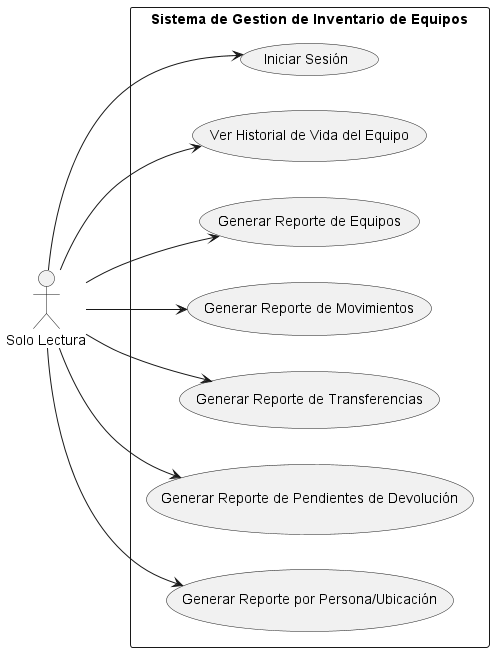
\includegraphics[scale=0.62]{./diagrams/CaseUses/ReadOnly/Solo Lectura.pdf}
\end{figure}
\begin{figure}[H]
    \centering
    \caption{Casos de Uso del Rol Administrador}\label{admin}
    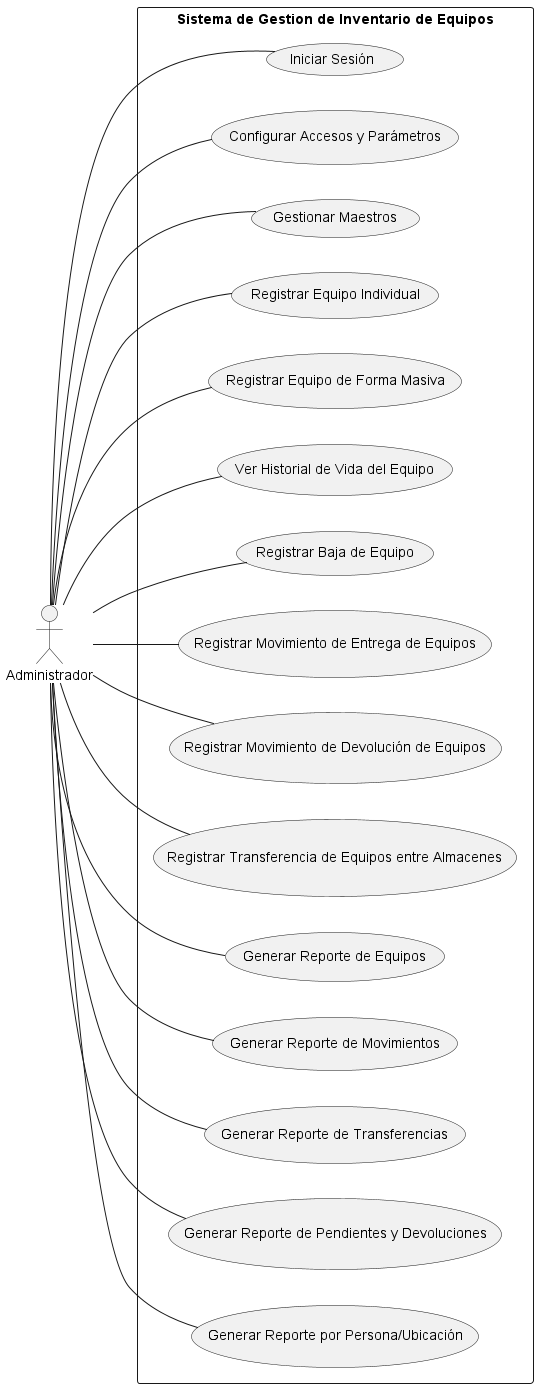
\includegraphics[scale=0.43]{./diagrams/CaseUses/Admin/Administrador.pdf}
\end{figure}
\subsubsection{Especificaci\'on de Casos de Uso}
Ahora se detallar\'an las especificaciones de cada uno de los casos de uso identificados anteriormente. Estas especificaciones proporcionan una descripci\'on precisa y estructurada de las interacciones entre los actores y el sistema, destacando los flujos
de eventos principales, las precondiciones, postcondiciones, y las excepciones relevantes. La especificaci\'on de casos de uso es esencial para guiar el dise\~{n}o y desarrollo del m\'odulo, asegurando que todas las funcionalidades requeridas est\'en claramente
definidas y alineadas con los objetivos del sistema.
\newline
\begin{longtable}{@{} p{16.5cm} @{}}
    \caption{Especificaci\'on de Caso de Uso Iniciar Sesi\'on}\label{tab:UC01}                                                                \\ \toprule
    \multicolumn{1}{c}{Caso de uso: Iniciar Sesi\'on}                                                                                         \\ \midrule
    ID:~UC01                                                                                                                                  \\ \midrule
    Breve descripci\'on:                                                                                                                      \\
    El usuario se autentica en el sistema utilizando sus credenciales del ERP de NextSoft.                                                    \\ \midrule
    Actores principales:                                                                                                                      \\
    Usuario (Administrador, Solo Lectura)                                                                                                     \\ \midrule
    Actores secundarios:                                                                                                                      \\
    Ninguno                                                                                                                                   \\ \midrule
    Precondiciones:                                                                                                                           \\
    1. El usuario debe tener una cuenta activa en el ERP.                                                                                     \\ \midrule
    Flujo principal:                                                                                                                          \\
    1. El usuario navega a la pantalla de inicio de sesi\'on del m\'odulo de gesti\'on de inventario de equipos.                              \\
    2. El sistema muestra un formulario de inicio de sesi\'on donde el usuario ingresa sus credenciales (nombre de usuario y contrase\~{n}a). \\
    3. El usuario ingresa sus credenciales y presiona el bot\'on ``Iniciar Sesi\'on''.                                                        \\
    4. El sistema valida las credenciales proporcionadas.                                                                                     \\
    5. Si las credenciales son correctas, el sistema autentica al usuario y muestra una pantalla para que elija el almac\'en.                 \\
    6. Una vez elegido el almac\'en determina su rol (Administrador o Solo Lectura).                                                          \\
    7. El usuario es redirigido a la p\'agina principal del m\'odulo con los permisos correspondientes a su rol.                              \\ \midrule
    Postcondiciones:                                                                                                                          \\
    1. El usuario accede al m\'odulo con los permisos correspondientes a su rol.                                                              \\ \midrule
    Flujos alternativos:                                                                                                                      \\
    A1- Credenciales incorrectas:                                                                                                             \\
    \hspace{1cm}1. El sistema ERP de NextSoft detecta que las credenciales ingresadas no son correctas.                                       \\
    \hspace{1cm}2. El sistema muestra un mensaje de error indicando que las credenciales son inv\'alidas.                                     \\
    \hspace{1cm}3. El flujo retorna al paso 2 del flujo principal si el usuario decide intentar nuevamente.                                   \\ \bottomrule
\end{longtable}
\newpage
\begin{longtable}{@{} p{16.5cm} @{}}
    \caption{Especificaci\'on de Caso de Uso Configurar Accesos y Par\'ametros}\label{tab:UC02}                                                        \\ \toprule
    \multicolumn{1}{c}{Caso de uso: Configurar Accesos y Par\'ametros}                                                                                 \\ \midrule
    ID:~UC02                                                                                                                                           \\ \midrule
    Breve descripci\'on:                                                                                                                               \\
    El administrador configura los usuarios con acceso a los almacenes y define los par\'ametros del sistema.                                          \\ \midrule
    Actores principales:                                                                                                                               \\
    Administrador                                                                                                                                      \\ \midrule
    Actores secundarios:                                                                                                                               \\
    Ninguno                                                                                                                                            \\ \midrule
    Precondiciones:                                                                                                                                    \\
    1. El administrador debe haber iniciado sesi\'on.                                                                                                  \\ \midrule
    Flujo principal:                                                                                                                                   \\
    1. El administrador navega a la secci\'on de configuraci\'on del m\'odulo de gesti\'on de inventario de equipos.                                   \\
    2. El sistema muestra una interfaz con opciones para configurar accesos a almacenes y definir par\'ametros del sistema.                            \\
    3. El administrador selecciona la opci\'on para gestionar usuarios y asignar permisos de acceso a los almacenes.                                   \\
    4. El administrador elige los usuarios, define su rol (Administrador o Solo Lectura) y asigna los almacenes correspondientes.                      \\
    5. El administrador guarda los cambios realizados.                                                                                                 \\
    6. El sistema guarda la configuraci\'on de accesos en la base de datos y muestra un mensaje de confirmaci\'on.                                     \\
    7. A continuaci\'on, el administrador selecciona la opci\'on para definir par\'ametros generales del m\'odulo (p. ej., familia de productos.).     \\
    8. El administrador ajusta los par\'ametros necesarios y guarda los cambios.                                                                       \\
    9. El sistema guarda los par\'ametros en la base de datos y confirma la actualizaci\'on con un mensaje de \'exito.                                 \\ \midrule
    Postcondiciones:                                                                                                                                   \\
    1. Los usuarios y par\'ametros son configurados correctamente y guardados en el sistema.                                                           \\ \midrule
    Flujos alternativos:                                                                                                                               \\
    A1- Error al guardar configuraciones:                                                                                                              \\
    \hspace{1cm}1. Si ocurre un error durante el guardado de los accesos o par\'ametros, el sistema muestra un mensaje de error indicando el problema. \\
    \hspace{1cm}2. El administrador tiene la opci\'on de intentar guardar nuevamente o revisar los cambios realizados.                                 \\
    \hspace{1cm}3. El flujo retorna al paso 5 o 8 del flujo principal, dependiendo de la acci\'on que decida tomar el administrador.                   \\ \bottomrule
\end{longtable}
\newpage
\begin{longtable}{@{} p{16.5cm} @{}}
    \caption{Especificaci\'on de Caso de Uso Gestionar Maestros}\label{tab:UC03}                                                                                                                  \\ \toprule
    \multicolumn{1}{c}{Caso de uso: Gestionar Maestros}                                                                                                                                           \\ \midrule
    ID:~UC03                                                                                                                                                                                      \\ \midrule
    Breve descripci\'on:                                                                                                                                                                          \\
    El usuario administra los datos maestros, como categor\'{\i}as, marcas, modelos, almacenes, proyectos, ubicaciones y atributos de equipos.                                                    \\ \midrule
    Actores principales:                                                                                                                                                                          \\
    Administrador                                                                                                                                                                                 \\ \midrule
    Actores secundarios:                                                                                                                                                                          \\
    Ninguno                                                                                                                                                                                       \\ \midrule
    Precondiciones:                                                                                                                                                                               \\
    1. El administrador debe haber iniciado sesi\'on.                                                                                                                                             \\ \midrule
    Flujo principal:                                                                                                                                                                              \\
    1. El administrador accede a la secci\'on de ``Maestros'' en el m\'odulo de gesti\'on de inventario de equipos.                                                                               \\
    2. El sistema muestra una lista de opciones para administrar diferentes tipos de datos maestros (categor\'{\i}as, marcas, modelos, almacenes, proyectos, ubicaciones y atributos de equipos). \\
    3. El administrador selecciona una de las opciones para gestionar los datos maestros.                                                                                                         \\
    4. El sistema muestra una lista con los registros existentes para el tipo de dato maestro seleccionado.                                                                                       \\
    5. El administrador puede realizar las siguientes acciones:                                                                                                                                   \\
    \hspace{1cm}- Registrar un nuevo dato maestro: El administrador introduce la informaci\'on requerida en un formulario y guarda el nuevo registro.                                             \\
    \hspace{1cm}- Actualizar un dato maestro existente: El administrador selecciona un registro, edita la informaci\'on y guarda los cambios.                                                     \\
    \hspace{1cm}- Eliminar un dato maestro: El administrador selecciona un registro y lo elimina del sistema.                                                                                     \\
    6. El sistema guarda los cambios realizados (registro, actualizaci\'on o eliminaci\'on) en la base de datos y muestra un mensaje de confirmaci\'on.                                           \\
    7. El administrador puede repetir el proceso para otros datos maestros o salir de la secci\'on.                                                                                               \\ \midrule
    Postcondiciones:                                                                                                                                                                              \\
    1. Los datos maestros son registrados, actualizados o eliminados en el sistema.                                                                                                               \\ \midrule
    Flujos alternativos:                                                                                                                                                                          \\
    A1- Error al guardar cambios:                                                                                                                                                                 \\
    \hspace{1cm}1. Si ocurre un error al intentar registrar, actualizar o eliminar un dato maestro, el sistema muestra un mensaje de error indicando el problema.                                 \\
    \hspace{1cm}2. El administrador tiene la opci\'on de intentar la acci\'on nuevamente o revisar los cambios realizados.                                                                        \\
    \hspace{1cm}3. El flujo retorna al paso 5 del flujo principal, dependiendo de la acci\'on que decida tomar el administrador.                                                                  \\ \bottomrule
\end{longtable}
\newpage
\begin{longtable}{@{} p{16.5cm} @{}}
    \caption{Especificaci\'on de Caso de Uso Registrar Equipo Individual}\label{tab:UC04}                                                                                                                                                                                                      \\ \toprule
    \multicolumn{1}{c}{Caso de uso: Registrar Equipo Individual}                                                                                                                                                                                                                               \\ \midrule
    ID:~UC04                                                                                                                                                                                                                                                                                   \\ \midrule
    Breve descripci\'on:                                                                                                                                                                                                                                                                       \\
    El administrador registra un equipo en el sistema de forma individual.                                                                                                                                                                                                                     \\ \midrule
    Actores principales:                                                                                                                                                                                                                                                                       \\
    Administrador                                                                                                                                                                                                                                                                              \\ \midrule
    Actores secundarios:                                                                                                                                                                                                                                                                       \\
    Ninguno                                                                                                                                                                                                                                                                                    \\ \midrule
    Precondiciones:                                                                                                                                                                                                                                                                            \\
    1. El usuario debe haber iniciado sesi\'on y tener el rol de administrador en el almac\'en seleccionado.                                                                                                                                                                                   \\ \midrule
    Flujo principal:                                                                                                                                                                                                                                                                           \\
    1. El administrador accede a la secci\'on de ``Agregar un nuevo equipo'' en el m\'odulo de gesti\'on de inventario de equipos.                                                                                                                                                             \\
    2. El sistema muestra un formulario para el registro individual de un equipo, solicitando informaci\'on como los datos de la factura, categor\'{\i}a, producto, marca, modelo, n\'umero de serie, activo fijo, descripci\'on, fecha y detalle de garant\'{\i}a, atributos y calibraciones. \\
    3. El administrador completa el formulario con la informaci\'on del equipo.                                                                                                                                                                                                                \\
    4. El administrador revisa la informaci\'on ingresada y presiona el bot\'on ``Guardar''.                                                                                                                                                                                                   \\
    5. El sistema valida la informaci\'on proporcionada y guarda el nuevo equipo en la base de datos.                                                                                                                                                                                          \\
    6. Autom\'aticamente, el sistema genera un movimiento de ingreso vinculado al almac\'en correspondiente donde se registr\'o el equipo.                                                                                                                                                     \\
    7. El sistema muestra un mensaje de confirmaci\'on indicando que el equipo ha sido registrado exitosamente.                                                                                                                                                                                \\ \midrule
    Postcondiciones:                                                                                                                                                                                                                                                                           \\
    1. El equipo es registrado, y se genera un movimiento de ingreso asociado al almac\'en.                                                                                                                                                                                                    \\ \midrule
    Flujos alternativos:                                                                                                                                                                                                                                                                       \\
    A1- Informaci\'on inv\'alida o incompleta:                                                                                                                                                                                                                                                 \\
    \hspace{1cm}1. Si la informaci\'on ingresada por el administrador es inv\'alida o est\'a incompleta, el sistema muestra un mensaje de error indicando los campos que necesitan correcci\'on.                                                                                               \\
    \hspace{1cm}2. El administrador corrige la informaci\'on y vuelve a intentar el registro del equipo.                                                                                                                                                                                       \\
    \hspace{1cm}3. El flujo retorna al paso 4 del flujo principal.                                                                                                                                                                                                                             \\ \bottomrule
\end{longtable}
\newpage
\begin{longtable}{@{} p{16.5cm} @{}}
    \caption{Especificaci\'on de Caso de Uso Registrar Equipo de Forma Masiva}\label{tab:UC05}                                                                                      \\ \toprule
    \multicolumn{1}{c}{Caso de uso: Registrar Equipo de Forma Masiva}                                                                                                               \\ \midrule
    ID:~UC05                                                                                                                                                                        \\ \midrule
    Breve descripci\'on:                                                                                                                                                            \\
    El administrador carga un archivo EXCEL para registrar m\'ultiples equipos simult\'aneamente.                                                                                   \\ \midrule
    Actores principales:                                                                                                                                                            \\
    Administrador                                                                                                                                                                   \\ \midrule
    Actores secundarios:                                                                                                                                                            \\
    Ninguno                                                                                                                                                                         \\ \midrule
    Precondiciones:                                                                                                                                                                 \\
    1. El usuario debe haber iniciado sesi\'on y tener el rol de administrador en el almac\'en seleccionado.                                                                        \\
    2. El usuario debe descargar la plantilla EXCEL.                                                                                                                                \\
    3. El usuario debe llenar la plantilla EXCEL con los datos solicitados.                                                                                                         \\ \midrule
    Flujo principal:                                                                                                                                                                \\
    1. El administrador accede a la secci\'on de ``Agregar varios desde un EXCEL'' en el m\'odulo de gesti\'on de inventario de equipos.                                            \\
    2. El sistema muestra una opci\'on para cargar un archivo EXCEL con la informaci\'on de los equipos a registrar.                                                                \\
    3. El administrador selecciona el archivo EXCEL desde su dispositivo y lo carga en el sistema.                                                                                  \\
    4. El sistema procesa el archivo, validando que la informaci\'on est\'e completa y sea correcta (e.g., formato correcto de n\'umero de serie, categor\'{\i}as v\'alidas, etc.). \\
    5. Si el archivo es v\'alido, el sistema muestra la lista de equipos procesados desde el EXCEL.                                                                                 \\
    6. El administrador revisa la informaci\'on y presiona el bot\'on ``Guardar''.                                                                                                  \\
    7. Autom\'aticamente, el sistema genera movimientos de ingreso para cada equipo registrado, vinculados al almac\'en correspondiente.                                            \\
    8. El sistema muestra un mensaje de confirmaci\'on indicando que los equipos han sido registrados exitosamente.                                                                 \\ \midrule
    Postcondiciones:                                                                                                                                                                \\
    1. Los equipos son registrados masivamente, y se generan los movimientos de ingreso correspondientes.                                                                           \\ \midrule
    Flujos alternativos:                                                                                                                                                            \\
    A1- Archivo EXCEL inv\'alido o informaci\'on incorrecta:                                                                                                                        \\
    \hspace{1cm}1. Si el archivo EXCEL tiene un formato incorrecto o contiene informaci\'on inv\'alida, el sistema muestra un mensaje de error.                                     \\
    \hspace{1cm}2. El administrador corrige el archivo y lo carga nuevamente en el sistema.                                                                                         \\
    \hspace{1cm}3. El flujo retorna al paso 3 del flujo principal.                                                                                                                  \\ \bottomrule
\end{longtable}
\newpage
\begin{longtable}{@{} p{16.5cm} @{}}
    \caption{Especificaci\'on de Caso de Uso Ver Historial de Vida del Equipo}\label{tab:UC06}                                                                                             \\ \toprule
    \multicolumn{1}{c}{Caso de uso: Ver Historial de Vida del Equipo}                                                                                                                      \\ \midrule
    ID:~UC06                                                                                                                                                                               \\ \midrule
    Breve descripci\'on:                                                                                                                                                                   \\
    El usuario visualiza el historial de vida de un equipo.                                                                                                                                \\ \midrule
    Actores principales:                                                                                                                                                                   \\
    Administrador, Solo Lectura                                                                                                                                                            \\ \midrule
    Actores secundarios:                                                                                                                                                                   \\
    Ninguno                                                                                                                                                                                \\ \midrule
    Precondiciones:                                                                                                                                                                        \\
    1. El usuario debe haber iniciado sesi\'on.                                                                                                                                            \\ \midrule
    Flujo principal:                                                                                                                                                                       \\
    1. El usuario accede a la secci\'on de ``Ver historial'' en el m\'odulo de gesti\'on de inventario de equipos.                                                                         \\
    2. El sistema recupera la informaci\'on del equipo seleccionado de la base de datos, incluyendo todos los cambios de estado (e.g., disponible, baja, mantenimiento, asignado).         \\
    3. El sistema muestra el historial completo del equipo en un modal, organizado de manera cronol\'ogica.                                                                                \\
    4. El usuario puede revisar el historial detallado, ver cada evento o cambio de estado con su fecha correspondiente, y obtener un panorama completo de la vida \'util del equipo.      \\ \midrule
    Postcondiciones:                                                                                                                                                                       \\
    1. El historial del equipo es mostrado en la pantalla.                                                                                                                                 \\ \midrule
    Flujos alternativos:                                                                                                                                                                   \\
    A1- Equipo no encontrado:                                                                                                                                                              \\
    \hspace{1cm}1. Si el equipo no se encuentra en la base de datos, el sistema muestra un mensaje de error, indicando que no se han encontrado resultados para el equipo seleccionado.    \\
    \hspace{1cm}2. El flujo retorna al paso 1 del flujo principal si se realiza una nueva b\'usqueda.                                                                                      \\
    A2- Error al recuperar datos del historial:                                                                                                                                            \\
    \hspace{1cm}1. Si ocurre un error al intentar recuperar los datos del historial del equipo, el sistema muestra un mensaje de error indicando el problema.                              \\
    \hspace{1cm}2. Si el problema persiste, el usuario puede contactar al soporte t\'ecnico para asistencia. El flujo puede continuar con una nueva b\'usqueda o finalizar el caso de uso. \\ \bottomrule
\end{longtable}
\newpage
\begin{longtable}{@{} p{16.5cm} @{}}
    \caption{Especificaci\'on de Caso de Uso Registrar Baja de Equipo}\label{tab:UC07}                                                                                                                                                  \\ \toprule
    \multicolumn{1}{c}{Caso de uso: Registrar Baja de Equipo}                                                                                                                                                                           \\ \midrule
    ID:~UC07                                                                                                                                                                                                                            \\ \midrule
    Breve descripci\'on:                                                                                                                                                                                                                \\
    El administrador registra la baja de un equipo, especificando el motivo.                                                                                                                                                            \\ \midrule
    Actores principales:                                                                                                                                                                                                                \\
    Administrador                                                                                                                                                                                                                       \\ \midrule
    Actores secundarios:                                                                                                                                                                                                                \\
    Ninguno                                                                                                                                                                                                                             \\ \midrule
    Precondiciones:                                                                                                                                                                                                                     \\
    1. El usuario debe haber iniciado sesi\'on y tener el rol de administrador en el almac\'en seleccionado.                                                                                                                            \\
    2. El equipo debe estar en estado ``Disponible''.                                                                                                                                                                                   \\ \midrule
    Flujo principal:                                                                                                                                                                                                                    \\
    1. El administrador accede a la secci\'on de ``Equipos'' en el m\'odulo de gesti\'on de inventario de equipos.                                                                                                                      \\
    2. El administrador selecciona el equipo que ser\'a dado de baja.                                                                                                                                                                   \\
    3. El administrador especifica el motivo de la baja para el equipo seleccionado.                                                                                                                                                    \\
    4. El administrador confirma la baja del equipo.                                                                                                                                                                                    \\
    5. El sistema verifica que el equipo seleccionado est\'a actualmente en el almac\'en y en un estado que permite la baja (e.g., ``Disponible'').                                                                                     \\
    6. El sistema actualiza el estado del equipo en la base de datos, cambi\'andolo a ``Baja'', junto con el motivo especificado.                                                                                                       \\                                                                                                                     \\
    8. El sistema muestra una confirmaci\'on de que la baja del equipo se ha registrado correctamente.                                                                                                                                  \\ \midrule
    Postcondiciones:                                                                                                                                                                                                                    \\
    1. El equipo es dado de baja, y se actualiza su estado a ``Baja'' en el sistema.                                                                                                                                                    \\ \midrule
    Flujos alternativos:                                                                                                                                                                                                                \\
    A1- Equipo no disponible para baja:                                                                                                                                                                                                 \\
    \hspace{1cm}1. Si el equipo seleccionado no est\'a disponible para la baja (e.g., en estado ``Asignado'', ``Mantenimiento'' o ya dado de baja), el sistema muestra un mensaje de error indicando que no se puede completar la baja. \\
    \hspace{1cm}3. El flujo retorna al paso 2 del flujo principal.                                                                                                                                                                      \\
    A2- Error en la base de datos:                                                                                                                                                                                                      \\
    \hspace{1cm}1. Si ocurre un error al intentar actualizar el estado del equipo o registrar la baja en la base de datos, el sistema muestra un mensaje de error indicando el problema.                                                \\
    \hspace{1cm}2. El administrador puede intentar registrar nuevamente la baja, o contactar al soporte t\'ecnico si el problema persiste.                                                                                              \\
    \hspace{1cm}3. El flujo puede continuar con una nueva tentativa de registro o finalizar el caso de uso.                                                                                                                             \\ \bottomrule
\end{longtable}
\newpage
\begin{longtable}{@{} p{16.5cm} @{}}
    \caption{Especificaci\'on de Caso de Uso Registrar Movimiento de Entrega de Equipos}\label{tab:UC08}                                                                                                                     \\ \toprule
    \multicolumn{1}{c}{Caso de uso: Registrar Movimiento de Entrega de Equipos}                                                                                                                                              \\ \midrule
    ID:~UC08                                                                                                                                                                                                                 \\ \midrule
    Breve descripci\'on:                                                                                                                                                                                                     \\
    El administrador registra la entrega de uno o varios equipos a un responsable.                                                                                                                                           \\ \midrule
    Actores principales:                                                                                                                                                                                                     \\
    Administrador                                                                                                                                                                                                            \\ \midrule
    Actores secundarios:                                                                                                                                                                                                     \\
    Ninguno                                                                                                                                                                                                                  \\ \midrule
    Precondiciones:                                                                                                                                                                                                          \\
    1. El usuario debe haber iniciado sesi\'on y tener el rol de administrador en el almac\'en seleccionado.                                                                                                                 \\ \midrule
    Flujo principal:                                                                                                                                                                                                         \\
    1. El administrador accede a la secci\'on de ``Registrar entrega'' en el m\'odulo de gesti\'on de inventario de equipos.                                                                                                 \\
    2. El administrador selecciona uno o varios equipos que ser\'an entregados.                                                                                                                                              \\
    3. El administrador asigna un responsable o una ubicaci\'on para los equipos seleccionados, adem\'as de un proyecto, sector y un motivo.                                                                                 \\
    4. El sistema verifica que los equipos seleccionados est\'en disponibles (estado ``Disponible'').                                                                                                                        \\
    5. El administrador confirma la entrega de los equipos.                                                                                                                                                                  \\
    6. El sistema actualiza el estado de los equipos a ``Asignado'' y registra el movimiento de entrega en la base de datos, asoci\'andolo al responsable asignado.                                                          \\
    7. El sistema muestra una confirmaci\'on de que la entrega se ha registrado correctamente.                                                                                                                               \\
    8. El administrador puede visualizar un resumen de la entrega o registrar una nueva entrega.                                                                                                                             \\ \midrule
    Postcondiciones:                                                                                                                                                                                                         \\
    1. El resumen de la entrega es mostrado en la pantalla.                                                                                                                                                                  \\ \midrule
    Flujos alternativos:                                                                                                                                                                                                     \\
    A1- Equipo no disponible:                                                                                                                                                                                                \\
    \hspace{1cm}1. Si alguno de los equipos seleccionados no est\'a disponible (e.g., ya asignado, en mantenimiento, o dado de baja), el sistema muestra un mensaje de error indicando que no se puede completar la entrega. \\
    \hspace{1cm}2. El administrador puede optar por deseleccionar los equipos no disponibles y continuar con la entrega de los equipos restantes.                                                                            \\
    \hspace{1cm}3. El flujo retorna al paso 5 del flujo principal si el administrador decide continuar.                                                                                                                      \\
    A2- Error en la base de datos:                                                                                                                                                                                           \\
    \hspace{1cm}1. Si ocurre un error al intentar actualizar el estado de los equipos o registrar el movimiento de entrega en la base de datos, el sistema muestra un mensaje de error indicando el problema.                \\
    \hspace{1cm}2. El administrador puede intentar registrar nuevamente la entrega, o contactar al soporte t\'ecnico si el problema persiste.                                                                                \\
    \hspace{1cm}3. El flujo puede continuar con una nueva tentativa de registro o finalizar el caso de uso.                                                                                                                  \\ \bottomrule
\end{longtable}
\newpage
\begin{longtable}{@{} p{16.5cm} @{}}
    \caption{Especificaci\'on de Caso de Uso Registrar Movimiento de Devoluci\'on de Equipos}\label{tab:UC09}                                                                                                                            \\ \toprule
    \multicolumn{1}{c}{Caso de uso: Registrar Movimiento de Devoluci\'on de Equipos}                                                                                                                                                     \\ \midrule
    ID:~UC09                                                                                                                                                                                                                             \\ \midrule
    Breve descripci\'on:                                                                                                                                                                                                                 \\
    El administrador registra la devoluci\'on de uno o varios equipos al almac\'en.                                                                                                                                                      \\ \midrule
    Actores principales:                                                                                                                                                                                                                 \\
    Administrador                                                                                                                                                                                                                        \\ \midrule
    Actores secundarios:                                                                                                                                                                                                                 \\
    Ninguno                                                                                                                                                                                                                              \\ \midrule
    Precondiciones:                                                                                                                                                                                                                      \\
    1. El usuario debe haber iniciado sesi\'on y tener el rol de administrador en el almac\'en seleccionado.                                                                                                                             \\
    2. El usuario debe haber seleccionado los equipos a devolver.                                                                                                                                                                        \\
    3. Los equipos seleccionados deben tener a un solo responsable.                                                                                                                                                                      \\ \midrule
    Flujo principal:                                                                                                                                                                                                                     \\
    1. El administrador accede a la secci\'on de ``Registrar devoluci\'on'' en el m\'odulo de gesti\'on de inventario de equipos.                                                                                                        \\
    2. El administrador escribe el motivo de la devoluci\'on de los equipos.                                                                                                                                                             \\
    3. El administrador confirma el estado f\'{\i}sico del equipo y escribe una observaci\'on por cada equipo si fuera necesario.                                                                                                        \\
    4. El sistema verifica que los equipos seleccionados est\'an actualmente asignados (estado ``Asignado'').                                                                                                                            \\
    5. El administrador confirma la devoluci\'on de los equipos.                                                                                                                                                                         \\
    6. El sistema actualiza el estado de los equipos a ``Disponible'' y registra el movimiento de devoluci\'on en la base de datos, liberando la asignaci\'on al responsable anterior.                                                   \\
    7. El sistema muestra una confirmaci\'on de que la devoluci\'on se ha registrado correctamente.                                                                                                                                      \\
    8. El administrador puede visualizar un resumen de la devoluci\'on o registrar una nueva devoluci\'on.                                                                                                                               \\ \midrule
    Postcondiciones:                                                                                                                                                                                                                     \\
    1. Los equipos son devueltos, y se actualiza el estado a ``Activo''.                                                                                                                                                                 \\ \midrule
    Flujos alternativos:                                                                                                                                                                                                                 \\
    A1- Equipo no asignado:                                                                                                                                                                                                              \\
    \hspace{1cm}1. Si alguno de los equipos seleccionados no est\'a asignado (e.g., ya en estado ``Activo'', ``Baja'', o ``Mantenimiento''), el sistema muestra un mensaje de error indicando que no se puede completar la devoluci\'on. \\
    \hspace{1cm}3. El flujo retorna al paso 1 del flujo principal.                                                                                                                                                                       \\
    A2- Error en la base de datos:                                                                                                                                                                                                       \\
    \hspace{1cm}1. Si ocurre un error al intentar actualizar el estado de los equipos o registrar el movimiento de devoluci\'on en la base de datos, el sistema muestra un mensaje de error indicando el problema.                       \\
    \hspace{1cm}2. El administrador puede intentar registrar nuevamente la devoluci\'on, o contactar al soporte t\'ecnico si el problema persiste.                                                                                       \\
    \hspace{1cm}3. El flujo puede continuar con una nueva tentativa de registro o finalizar el caso de uso.                                                                                                                              \\ \bottomrule
\end{longtable}
\newpage
\begin{longtable}{@{} p{16.5cm} @{}}
    \caption{Especificaci\'on de Caso de Uso Registrar Transferencia de Equipos entre Almacenes}\label{tab:UC010}                                                                                                                            \\ \toprule
    \multicolumn{1}{c}{Caso de uso: Registrar Transferencia de Equipos entre Almacenes}                                                                                                                                                      \\ \midrule
    ID:~UC010                                                                                                                                                                                                                                \\ \midrule
    Breve descripci\'on:                                                                                                                                                                                                                     \\
    El administrador transfiere uno o varios equipos de un almac\'en a otro.                                                                                                                                                                 \\ \midrule
    Actores principales:                                                                                                                                                                                                                     \\
    Administrador                                                                                                                                                                                                                            \\ \midrule
    Actores secundarios:                                                                                                                                                                                                                     \\
    Ninguno                                                                                                                                                                                                                                  \\ \midrule
    Precondiciones:                                                                                                                                                                                                                          \\
    1. El usuario debe haber iniciado sesi\'on y tener el rol de administrador en el almac\'en seleccionado (origen).                                                                                                                        \\ \midrule
    Flujo principal:                                                                                                                                                                                                                         \\
    1. El administrador accede a la secci\'on de ``Registrar transferencia'' en el m\'odulo de gesti\'on de inventario de equipos.                                                                                                           \\
    2. El administrador selecciona el almac\'en de destino para la transferencia.                                                                                                                                                            \\
    3. El administrador selecciona uno o varios equipos que ser\'an transferidos del almac\'en de origen al almac\'en de destino.                                                                                                            \\
    4. El administrador confirma la transferencia de los equipos.                                                                                                                                                                            \\
    5. El sistema verifica que los equipos seleccionados est\'an actualmente en el almac\'en de origen y en un estado que permite la transferencia (e.g., ``Disponible'').                                                                   \\
    6. El sistema actualiza el estado de los equipos en la base de datos, registrando la salida del almac\'en de origen y la entrada en el almac\'en de destino.                                                                             \\
    7. El sistema genera los movimientos correspondientes en la base de datos, registrando la transferencia para cada equipo.                                                                                                                \\
    8. El sistema muestra una confirmaci\'on de que la transferencia se ha registrado correctamente.                                                                                                                                         \\
    9. El administrador puede visualizar un resumen de la transferencia o registrar una nueva transferencia.                                                                                                                                 \\ \midrule
    Postcondiciones:                                                                                                                                                                                                                         \\
    1. Los equipos son transferidos, y se generan los movimientos correspondientes en el sistema.                                                                                                                                            \\ \midrule
    Flujos alternativos:                                                                                                                                                                                                                     \\
    A1- Equipo no disponible para trasferencia:                                                                                                                                                                                              \\
    \hspace{1cm}1. Si alguno de los equipos seleccionados no est\'a disponible para la transferencia (e.g., en estado ``Baja'' o ``Asignado''), el sistema muestra un mensaje de error indicando que no se puede completar la transferencia. \\
    \hspace{1cm}2. El administrador puede optar por deseleccionar los equipos no transferibles y continuar con la transferencia de los equipos restantes.                                                                                    \\
    \hspace{1cm}3. El flujo retorna al paso 5 del flujo principal si el administrador decide continuar.                                                                                                                                      \\
    A2- Error en la base de datos:                                                                                                                                                                                                           \\
    \hspace{1cm}1. Si ocurre un error al intentar registrar los movimientos de transferencia en la base de datos, el sistema muestra un mensaje de error indicando el problema.                                                              \\
    \hspace{1cm}2. El administrador puede intentar registrar nuevamente la transferencia, o contactar al soporte t\'ecnico si el problema persiste.                                                                                          \\
    \hspace{1cm}3. El flujo puede continuar con una nueva tentativa de registro o finalizar el caso de uso.                                                                                                                                  \\ \bottomrule
\end{longtable}
\newpage
\begin{longtable}{@{} p{16.5cm} @{}}
    \caption{Especificaci\'on de Caso de Uso Generar Reporte de Equipos}\label{tab:UC011}                                                                                                                                                                                        \\ \toprule
    \multicolumn{1}{c}{Caso de uso: Generar Reporte de Equipos}                                                                                                                                                                                                                  \\ \midrule
    ID:~UC011                                                                                                                                                                                                                                                                    \\ \midrule
    Breve descripci\'on:                                                                                                                                                                                                                                                         \\
    El usuario genera un reporte que muestra todos los equipos registrados en el sistema, filtrando por categor\'{\i}a, marca, equipo, estado, entre otros criterios.                                                                                                            \\ \midrule
    Actores principales:                                                                                                                                                                                                                                                         \\
    Administrador, Solo Lectura                                                                                                                                                                                                                                                  \\ \midrule
    Actores secundarios:                                                                                                                                                                                                                                                         \\
    Ninguno                                                                                                                                                                                                                                                                      \\ \midrule
    Precondiciones:                                                                                                                                                                                                                                                              \\
    1. El usuario debe haber iniciado sesi\'on.                                                                                                                                                                                                                                  \\ \midrule
    Flujo principal:                                                                                                                                                                                                                                                             \\
    1. El usuario accede a la secci\'on de ``Reporte de equipos'' en el m\'odulo de gesti\'on de inventario de equipos.                                                                                                                                                          \\
    2. El sistema presenta una interfaz en la que el usuario puede seleccionar los filtros deseados, como estado del equipo, categor\'{\i}a, fechas, entre otros.                                                                                                                \\
    3. El usuario selecciona los criterios de filtrado y el formato de exportaci\'on del reporte (e.g., Excel, Listado).                                                                                                                                                         \\
    4. El usuario confirma la generaci\'on del reporte.                                                                                                                                                                                                                          \\
    5. El sistema consulta la base de datos para recuperar la informaci\'on de los equipos que cumplen con los criterios de filtrado especificados.                                                                                                                              \\
    6. El sistema genera el reporte con la informaci\'on obtenida, present\'andolo en pantalla para su revisi\'on.                                                                                                                                                               \\
    7. Si el usuario seleccion\'o un formato de exportaci\'on, el sistema genera un archivo en el formato especificado.                                                                                                                                                          \\
    8. El usuario revisa el reporte y puede optar por guardarlo, imprimirlo o realizar una nueva consulta.                                                                                                                                                                       \\ \midrule
    Postcondiciones:                                                                                                                                                                                                                                                             \\
    1. El reporte es generado y presentado en pantalla o exportado en un formato seleccionable (e.g., Excel).                                                                                                                                                                    \\ \midrule
    Flujos alternativos:                                                                                                                                                                                                                                                         \\
    A1- Filtros inv\'alidos o sin resultados:                                                                                                                                                                                                                                    \\
    \hspace{1cm}1. Si el usuario selecciona un conjunto de filtros que no devuelve ning\'un resultado (e.g., no hay equipos que coincidan con los criterios seleccionados), el sistema muestra un mensaje informando que no se encontraron datos para los filtros seleccionados. \\
    \hspace{1cm}2. El usuario puede optar por modificar los filtros y realizar una nueva consulta.                                                                                                                                                                               \\
    \hspace{1cm}3. El flujo retorna al paso 3 del flujo principal si el usuario decide ajustar los filtros.                                                                                                                                                                      \\
    A2- Error en la generaci\'on del reporte:                                                                                                                                                                                                                                    \\
    \hspace{1cm}1. Si ocurre un error durante la generaci\'on del reporte (e.g., problemas con la conexi\'on a la base de datos o error en la exportaci\'on del archivo), el sistema muestra un mensaje de error indicando la naturaleza del problema.                           \\
    \hspace{1cm}2. El usuario puede intentar generar el reporte nuevamente, seleccionar un conjunto de filtros diferente, o contactar al soporte t\'ecnico si el problema persiste.                                                                                              \\
    \hspace{1cm}3. El flujo puede continuar con una nueva tentativa de generaci\'on o finalizar el caso de uso.                                                                                                                                                                  \\ \bottomrule
\end{longtable}
\newpage
\begin{longtable}{@{} p{16.5cm} @{}}
    \caption{Especificaci\'on de Caso de Uso Generar Reporte de Movimientos}\label{tab:UC012}                                                                                                                                                                                        \\ \toprule
    \multicolumn{1}{c}{Caso de uso: Generar Reporte de Movimientos}                                                                                                                                                                                                                  \\ \midrule
    ID:~UC012                                                                                                                                                                                                                                                                        \\ \midrule
    Breve descripci\'on:                                                                                                                                                                                                                                                             \\
    El usuario genera un reporte detallado de los movimientos de equipos, incluyendo entregas, devoluciones y transferencias.                                                                                                                                                        \\ \midrule
    Actores principales:                                                                                                                                                                                                                                                             \\
    Administrador, Solo Lectura                                                                                                                                                                                                                                                      \\ \midrule
    Actores secundarios:                                                                                                                                                                                                                                                             \\
    Ninguno                                                                                                                                                                                                                                                                          \\ \midrule
    Precondiciones:                                                                                                                                                                                                                                                                  \\
    1. El usuario debe haber iniciado sesi\'on.                                                                                                                                                                                                                                      \\ \midrule
    Flujo principal:                                                                                                                                                                                                                                                                 \\
    1. El usuario accede a la secci\'on de ``Reporte de movimientos'' en el m\'odulo de gesti\'on de inventario de equipos.                                                                                                                                                          \\
    2. El sistema presenta una interfaz en la que el usuario puede seleccionar los filtros deseados, como tipo de movimiento, responsable, almac\'en, categor\'{\i}a, fechas, entre otros.                                                                                           \\
    3. El usuario selecciona los criterios de filtrado y el formato de exportaci\'on del reporte (e.g., Excel, Listado).                                                                                                                                                             \\
    4. El usuario confirma la generaci\'on del reporte.                                                                                                                                                                                                                              \\
    5. El sistema consulta la base de datos para recuperar la informaci\'on de los movimientos que cumplen con los criterios de filtrado especificados.                                                                                                                              \\
    6. El sistema genera el reporte con la informaci\'on obtenida, present\'andolo en pantalla para su revisi\'on.                                                                                                                                                                   \\
    7. Si el usuario seleccion\'o un formato de exportaci\'on, el sistema genera un archivo en el formato especificado.                                                                                                                                                              \\
    8. El usuario revisa el reporte y puede optar por guardarlo, imprimirlo o realizar una nueva consulta.                                                                                                                                                                           \\ \midrule
    Postcondiciones:                                                                                                                                                                                                                                                                 \\
    1. El reporte es generado y presentado en pantalla o exportado en un formato seleccionable (e.g., Excel).                                                                                                                                                                        \\ \midrule
    Flujos alternativos:                                                                                                                                                                                                                                                             \\
    A1- Filtros inv\'alidos o sin resultados:                                                                                                                                                                                                                                        \\
    \hspace{1cm}1. Si el usuario selecciona un conjunto de filtros que no devuelve ning\'un resultado (e.g., no hay movimientos que coincidan con los criterios seleccionados), el sistema muestra un mensaje informando que no se encontraron datos para los filtros seleccionados. \\
    \hspace{1cm}2. El usuario puede optar por modificar los filtros y realizar una nueva consulta.                                                                                                                                                                                   \\
    \hspace{1cm}3. El flujo retorna al paso 3 del flujo principal si el usuario decide ajustar los filtros.                                                                                                                                                                          \\
    A2- Error en la generaci\'on del reporte:                                                                                                                                                                                                                                        \\
    \hspace{1cm}1. Si ocurre un error durante la generaci\'on del reporte (e.g., problemas con la conexi\'on a la base de datos o error en la exportaci\'on del archivo), el sistema muestra un mensaje de error indicando la naturaleza del problema.                               \\
    \hspace{1cm}2. El usuario puede intentar generar el reporte nuevamente, seleccionar un conjunto de filtros diferente, o contactar al soporte t\'ecnico si el problema persiste.                                                                                                  \\
    \hspace{1cm}3. El flujo puede continuar con una nueva tentativa de generaci\'on o finalizar el caso de uso.                                                                                                                                                                      \\ \bottomrule
\end{longtable}
\newpage
\begin{longtable}{@{} p{16.5cm} @{}}
    \caption{Especificaci\'on de Caso de Uso Generar Reporte de Transferencias}\label{tab:UC013}                                                                                                                                                                                        \\ \toprule
    \multicolumn{1}{c}{Caso de uso: Generar Reporte de Transferencias}                                                                                                                                                                                                                  \\ \midrule
    ID:~UC013                                                                                                                                                                                                                                                                           \\ \midrule
    Breve descripci\'on:                                                                                                                                                                                                                                                                \\
    El usuario genera un reporte detallado de las transferencias de equipos, filtrando por almac\'en de origen y almac\'en de destino.                                                                                                                                                  \\ \midrule
    Actores principales:                                                                                                                                                                                                                                                                \\
    Administrador, Solo Lectura                                                                                                                                                                                                                                                         \\ \midrule
    Actores secundarios:                                                                                                                                                                                                                                                                \\
    Ninguno                                                                                                                                                                                                                                                                             \\ \midrule
    Precondiciones:                                                                                                                                                                                                                                                                     \\
    1. El usuario debe haber iniciado sesi\'on.                                                                                                                                                                                                                                         \\ \midrule
    Flujo principal:                                                                                                                                                                                                                                                                    \\
    1. El usuario accede a la secci\'on de ``Reporte de transferencias'' en el m\'odulo de gesti\'on de inventario de equipos.                                                                                                                                                          \\
    2. El sistema presenta una interfaz en la que el usuario puede seleccionar los filtros deseados, como almac\'en de origen, almac\'en de destino y fechas.                                                                                                                           \\
    3. El usuario selecciona los criterios de filtrado y el formato de exportaci\'on del reporte (e.g., Excel, Listado).                                                                                                                                                                \\
    4. El usuario confirma la generaci\'on del reporte.                                                                                                                                                                                                                                 \\
    5. El sistema consulta la base de datos para recuperar la informaci\'on de las transferencias que cumplen con los criterios de filtrado especificados.                                                                                                                              \\
    6. El sistema genera el reporte con la informaci\'on obtenida, present\'andolo en pantalla para su revisi\'on.                                                                                                                                                                      \\
    7. Si el usuario seleccion\'o un formato de exportaci\'on, el sistema genera un archivo en el formato especificado.                                                                                                                                                                 \\
    8. El usuario revisa el reporte y puede optar por guardarlo, imprimirlo o realizar una nueva consulta.                                                                                                                                                                              \\ \midrule
    Postcondiciones:                                                                                                                                                                                                                                                                    \\
    1. El reporte es generado y presentado en pantalla o exportado en un formato seleccionable (e.g., Excel).                                                                                                                                                                           \\ \midrule
    Flujos alternativos:                                                                                                                                                                                                                                                                \\
    A1- Filtros inv\'alidos o sin resultados:                                                                                                                                                                                                                                           \\
    \hspace{1cm}1. Si el usuario selecciona un conjunto de filtros que no devuelve ning\'un resultado (e.g., no hay transferencias que coincidan con los criterios seleccionados), el sistema muestra un mensaje informando que no se encontraron datos para los filtros seleccionados. \\
    \hspace{1cm}2. El usuario puede optar por modificar los filtros y realizar una nueva consulta.                                                                                                                                                                                      \\
    \hspace{1cm}3. El flujo retorna al paso 3 del flujo principal si el usuario decide ajustar los filtros.                                                                                                                                                                             \\
    A2- Error en la generaci\'on del reporte:                                                                                                                                                                                                                                           \\
    \hspace{1cm}1. Si ocurre un error durante la generaci\'on del reporte (e.g., problemas con la conexi\'on a la base de datos o error en la exportaci\'on del archivo), el sistema muestra un mensaje de error indicando la naturaleza del problema.                                  \\
    \hspace{1cm}2. El usuario puede intentar generar el reporte nuevamente, seleccionar un conjunto de filtros diferente, o contactar al soporte t\'ecnico si el problema persiste.                                                                                                     \\
    \hspace{1cm}3. El flujo puede continuar con una nueva tentativa de generaci\'on o finalizar el caso de uso.                                                                                                                                                                         \\ \bottomrule
\end{longtable}
\newpage
\begin{longtable}{@{} p{16.5cm} @{}}
    \caption{Especificaci\'on de Caso de Uso Generar Reporte de Pendientes de Devoluci\'on}\label{tab:UC014}                                                                                                                                                                         \\ \toprule
    \multicolumn{1}{c}{Caso de uso: Generar Reporte de Pendientes de Devoluci\'on}                                                                                                                                                                                                   \\ \midrule
    ID:~UC014                                                                                                                                                                                                                                                                        \\ \midrule
    Breve descripci\'on:                                                                                                                                                                                                                                                             \\
    El usuario genera un reporte que lista los equipos devueltos y pendientes de devoluci\'on.                                                                                                                                                                                       \\ \midrule
    Actores principales:                                                                                                                                                                                                                                                             \\
    Administrador, Solo Lectura                                                                                                                                                                                                                                                      \\ \midrule
    Actores secundarios:                                                                                                                                                                                                                                                             \\
    Ninguno                                                                                                                                                                                                                                                                          \\ \midrule
    Precondiciones:                                                                                                                                                                                                                                                                  \\
    1. El usuario debe haber iniciado sesi\'on.                                                                                                                                                                                                                                      \\ \midrule
    Flujo principal:                                                                                                                                                                                                                                                                 \\
    1. El usuario accede a la secci\'on de ``Reporte de pendientes y devoluciones'' en el m\'odulo de gesti\'on de inventario de equipos.                                                                                                                                            \\
    2. El sistema presenta una interfaz en la que el usuario puede seleccionar los filtros deseados, como almac\'en, proyecto, sector, ubicaci\'on, responsable, tipo (pendiente o devuelto) y fechas.                                                                               \\
    3. El usuario selecciona los criterios de filtrado y el formato de exportaci\'on del reporte (e.g., Excel, Listado).                                                                                                                                                             \\
    4. El usuario confirma la generaci\'on del reporte.                                                                                                                                                                                                                              \\
    5. El sistema consulta la base de datos para recuperar la informaci\'on de los movimientos que cumplen con los criterios de filtrado especificados.                                                                                                                              \\
    6. El sistema genera el reporte con la informaci\'on obtenida, present\'andolo en pantalla para su revisi\'on.                                                                                                                                                                   \\
    7. Si el usuario seleccion\'o un formato de exportaci\'on, el sistema genera un archivo en el formato especificado.                                                                                                                                                              \\
    8. El usuario revisa el reporte y puede optar por guardarlo, imprimirlo o realizar una nueva consulta.                                                                                                                                                                           \\ \midrule
    Postcondiciones:                                                                                                                                                                                                                                                                 \\
    1. El reporte es generado y presentado en pantalla o exportado en un formato seleccionable (e.g., Excel).                                                                                                                                                                        \\ \midrule
    Flujos alternativos:                                                                                                                                                                                                                                                             \\
    A1- Filtros inv\'alidos o sin resultados:                                                                                                                                                                                                                                        \\
    \hspace{1cm}1. Si el usuario selecciona un conjunto de filtros que no devuelve ning\'un resultado (e.g., no hay movimientos que coincidan con los criterios seleccionados), el sistema muestra un mensaje informando que no se encontraron datos para los filtros seleccionados. \\
    \hspace{1cm}2. El usuario puede optar por modificar los filtros y realizar una nueva consulta.                                                                                                                                                                                   \\
    \hspace{1cm}3. El flujo retorna al paso 3 del flujo principal si el usuario decide ajustar los filtros.                                                                                                                                                                          \\
    A2- Error en la generaci\'on del reporte:                                                                                                                                                                                                                                        \\
    \hspace{1cm}1. Si ocurre un error durante la generaci\'on del reporte (e.g., problemas con la conexi\'on a la base de datos o error en la exportaci\'on del archivo), el sistema muestra un mensaje de error indicando la naturaleza del problema.                               \\
    \hspace{1cm}2. El usuario puede intentar generar el reporte nuevamente, seleccionar un conjunto de filtros diferente, o contactar al soporte t\'ecnico si el problema persiste.                                                                                                  \\
    \hspace{1cm}3. El flujo puede continuar con una nueva tentativa de generaci\'on o finalizar el caso de uso.                                                                                                                                                                      \\ \bottomrule
\end{longtable}
\newpage
\begin{longtable}{@{} p{16.5cm} @{}}
    \caption{Especificaci\'on de Caso de Uso Generar Reporte por Persona/Ubicaci\'on}\label{tab:UC015}                                                                                                                                                                           \\ \toprule
    \multicolumn{1}{c}{Caso de uso: Generar Reporte por Persona/Ubicaci\'on}                                                                                                                                                                                                     \\ \midrule
    ID:~UC015                                                                                                                                                                                                                                                                    \\ \midrule
    Breve descripci\'on:                                                                                                                                                                                                                                                         \\
    El usuario genera un reporte que muestra todos los equipos asignados a un trabajador espec\'{\i}fico o a una ubicaci\'on determinada.                                                                                                                                        \\ \midrule
    Actores principales:                                                                                                                                                                                                                                                         \\
    Administrador, Solo Lectura                                                                                                                                                                                                                                                  \\ \midrule
    Actores secundarios:                                                                                                                                                                                                                                                         \\
    Ninguno                                                                                                                                                                                                                                                                      \\ \midrule
    Precondiciones:                                                                                                                                                                                                                                                              \\
    1. El usuario debe haber iniciado sesi\'on.                                                                                                                                                                                                                                  \\ \midrule
    Flujo principal:                                                                                                                                                                                                                                                             \\
    1. El usuario accede a la secci\'on de ``Reporte de persona/ubicaci\'on'' en el m\'odulo de gesti\'on de inventario de equipos.                                                                                                                                              \\
    2. El sistema presenta una interfaz en la que el usuario puede seleccionar los filtros deseados, como ubicaci\'on, responsable o ambos.                                                                                                                                      \\
    3. El usuario selecciona los criterios de filtrado y el formato de exportaci\'on del reporte (e.g., Excel, Listado).                                                                                                                                                         \\
    4. El usuario confirma la generaci\'on del reporte.                                                                                                                                                                                                                          \\
    5. El sistema consulta la base de datos para recuperar la informaci\'on de los equipos que cumplen con los criterios de filtrado especificados.                                                                                                                              \\
    6. El sistema genera el reporte con la informaci\'on obtenida, present\'andolo en pantalla para su revisi\'on.                                                                                                                                                               \\
    7. Si el usuario seleccion\'o un formato de exportaci\'on, el sistema genera un archivo en el formato especificado.                                                                                                                                                          \\
    8. El usuario revisa el reporte y puede optar por guardarlo, imprimirlo o realizar una nueva consulta.                                                                                                                                                                       \\ \midrule
    Postcondiciones:                                                                                                                                                                                                                                                             \\
    1. El reporte es generado y presentado en pantalla o exportado en un formato seleccionable (e.g., Excel).                                                                                                                                                                    \\ \midrule
    Flujos alternativos:                                                                                                                                                                                                                                                         \\
    A1- Filtros inv\'alidos o sin resultados:                                                                                                                                                                                                                                    \\
    \hspace{1cm}1. Si el usuario selecciona un conjunto de filtros que no devuelve ning\'un resultado (e.g., no hay equipos que coincidan con los criterios seleccionados), el sistema muestra un mensaje informando que no se encontraron datos para los filtros seleccionados. \\
    \hspace{1cm}2. El usuario puede optar por modificar los filtros y realizar una nueva consulta.                                                                                                                                                                               \\
    \hspace{1cm}3. El flujo retorna al paso 3 del flujo principal si el usuario decide ajustar los filtros.                                                                                                                                                                      \\
    A2- Error en la generaci\'on del reporte:                                                                                                                                                                                                                                    \\
    \hspace{1cm}1. Si ocurre un error durante la generaci\'on del reporte (e.g., problemas con la conexi\'on a la base de datos o error en la exportaci\'on del archivo), el sistema muestra un mensaje de error indicando la naturaleza del problema.                           \\
    \hspace{1cm}2. El usuario puede intentar generar el reporte nuevamente, seleccionar un conjunto de filtros diferente, o contactar al soporte t\'ecnico si el problema persiste.                                                                                              \\
    \hspace{1cm}3. El flujo puede continuar con una nueva tentativa de generaci\'on o finalizar el caso de uso.                                                                                                                                                                  \\ \bottomrule
\end{longtable}
\newpage
\subsubsection{Diagramas de Clases}
\begin{figure}[H]
    \centering
    \caption{Entidades}
    \includegraphics[width=21cm, height=16.5cm, angle=90]{./diagrams/Classes/Entities/Entities.pdf}
\end{figure}
\begin{figure}[H]
    \centering
    \caption{DTO}
    \includegraphics[width=16.5cm, height=21cm, angle=0]{./diagrams/Classes/DTO/DTO.pdf}
\end{figure}
\begin{figure}[H]
    \centering
    \caption{L\'ogica de negocio}
    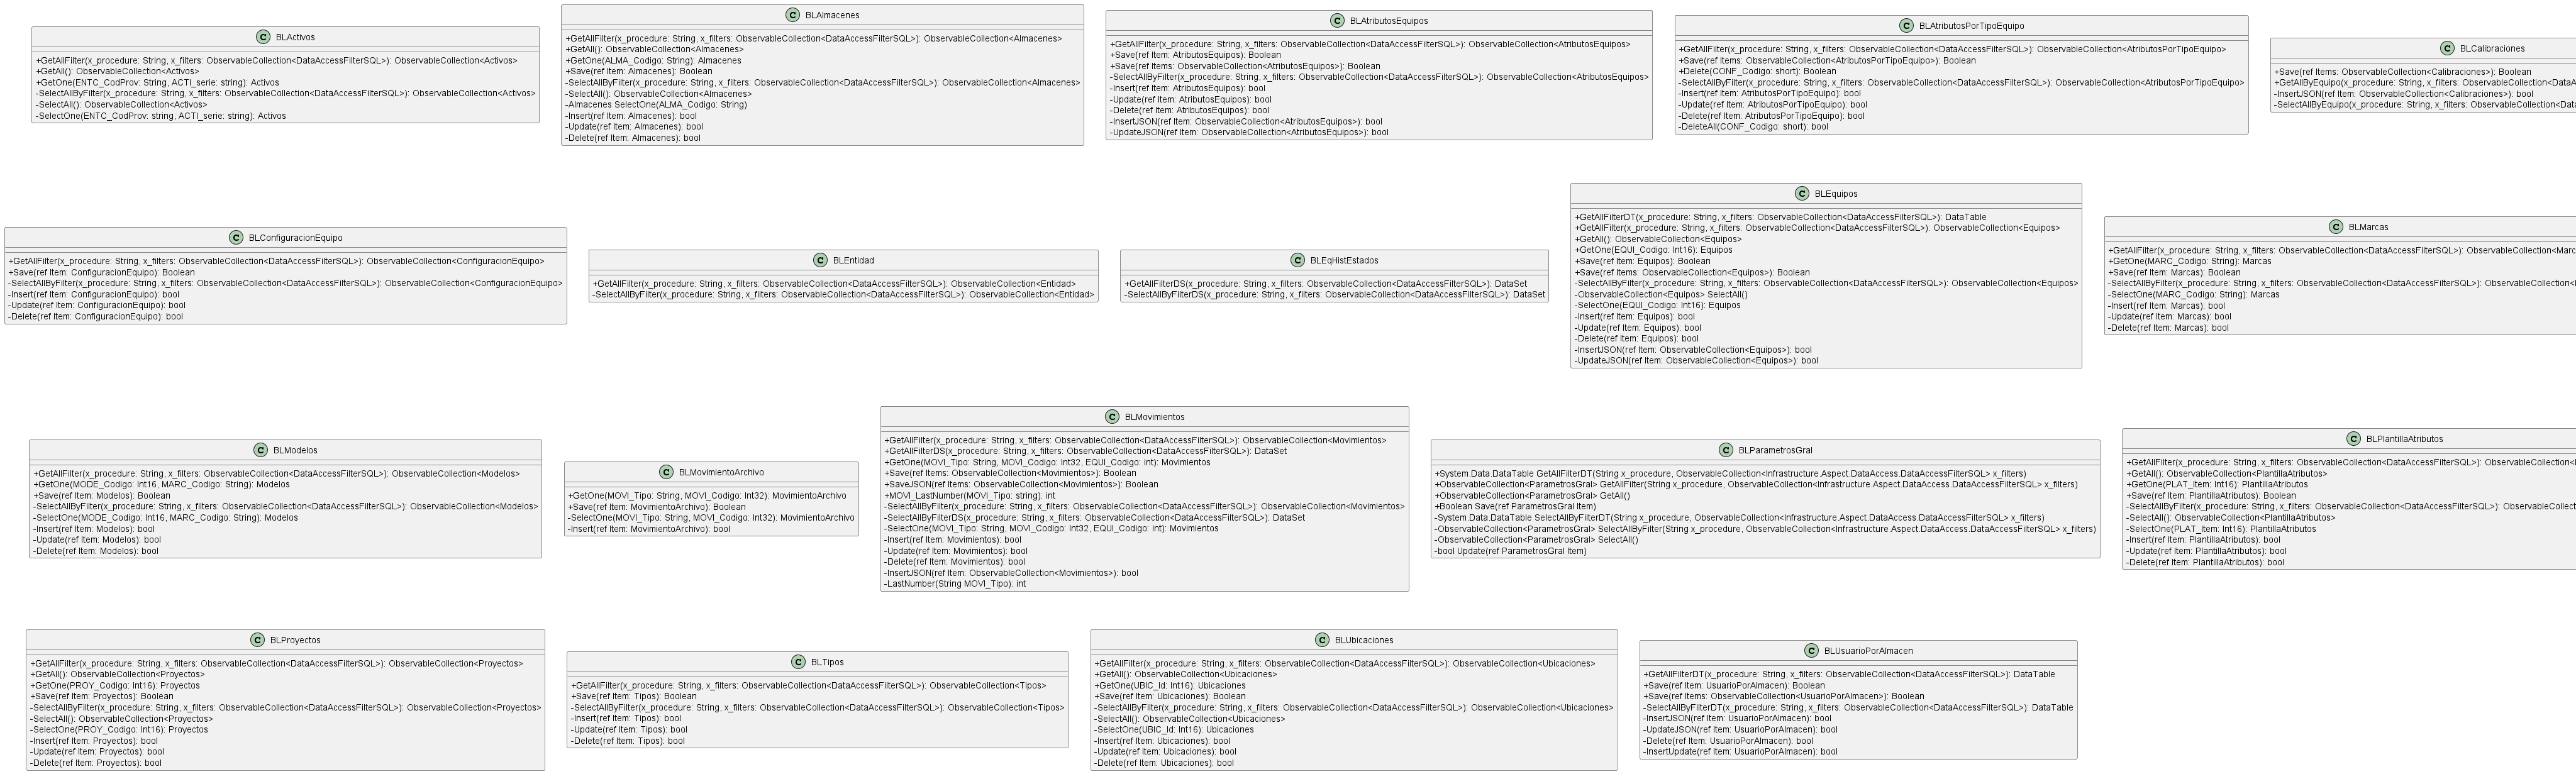
\includegraphics[width=21cm, height=16.5cm, angle=90]{./diagrams/Classes/BusinessLogic/BusinessLogic.pdf}
\end{figure}
\begin{figure}[H]
    \centering
    \caption{API}
    \includegraphics[width=21cm, height=16.5cm, angle=90]{./diagrams/Classes/Services/Service.pdf}
\end{figure}
\subsubsection{Diagrama de Entidad Relaci\'on}
\begin{figure}[H]
    \centering
    \caption{Base de datos}
    \includegraphics[width=21cm, height=16.5cm, angle=90]{./diagrams/ER/ER.pdf}
\end{figure}
\subsubsection{Diagramas de Secuencia}
\begin{figure}[H]
    \centering
    \caption{Registrar equipo individual}
    \includegraphics[width=21cm, height=16.5cm, angle=90]{./diagrams/Sequence/RegistrarEquipo/RegistrarEquipo.pdf}
\end{figure}
\begin{figure}[H]
    \centering
    \caption{Registrar equipo de forma masiva}
    \includegraphics[width=21cm, height=16.5cm, angle=90]{./diagrams/Sequence/RegistrarEquipoMasivo/RegistrarEquipoMasivo.pdf}
\end{figure}
\begin{figure}[H]
    \centering
    \caption{Registrar Movimiento de Entrega de Equipos y Registrar Transferencia de Equipos entre Almacenes}
    \includegraphics[width=21cm, height=16.5cm, angle=90]{./diagrams/Sequence/EntregaTransferencia/EntregaTransferencia.pdf}
\end{figure}
\begin{figure}[H]
    \centering
    \caption{Registrar Movimiento de Devoluci\'on de Equipos}
    \includegraphics[width=21cm, height=16.5cm, angle=90]{./diagrams/Sequence/RegistrarDevolucion/RegistrarDevolucion.pdf}
\end{figure}
\subsubsection{Interfaces}
El dise\~{n}o de la interfaz de usuario es crucial para garantizar que los usuarios puedan interactuar de manera eficiente y efectiva con el m\'odulo de gesti\'on de inventario de equipos. Ahora se presentar\'an mockups que representan las principales pantallas del m\'odulo. Estos dise\~{n}os ayudar\'an a visualizar la disposici\'on de los elementos en la interfaz y asegurar\'an que la experiencia del usuario sea intuitiva y coherente.

\textbf{Pantalla de Inicio de Sesi\'on (Figura~\ref{login}). }La pantalla de inicio de sesi\'on es la primera interacci\'on del usuario con el m\'odulo. En esta pantalla, el usuario debe ingresar sus credenciales del ERP de NextSoft para acceder al sistema. La interfaz es sencilla, con campos para el usuario y la contrase\~{n}a, y un bot\'on de inicio de sesi\'on.
\begin{figure}[H]
    \centering
    \caption{Inicio de Sesi\'on}\label{login}
    
\includegraphics[width=16.5cm, angle=0]{./images/login.png}
\end{figure}
\textbf{Pantalla de Registro Individual de Equipo (Figura~\ref{individual}). }Esta pantalla permite al administrador registrar un nuevo equipo en el sistema de forma individual. Incluye campos para ingresar detalles como el n\'umero de serie, modelo, marca, categor\'{\i}a, y otros atributos espec\'{\i}ficos del equipo. Una vez completado el formulario, el administrador puede guardar el registro y autom\'aticamente se generar\'a un movimiento de ingreso al almac\'en correspondiente.
\begin{figure}[H]
    \centering
    \caption{Registrar Equipo Individual}\label{individual}
    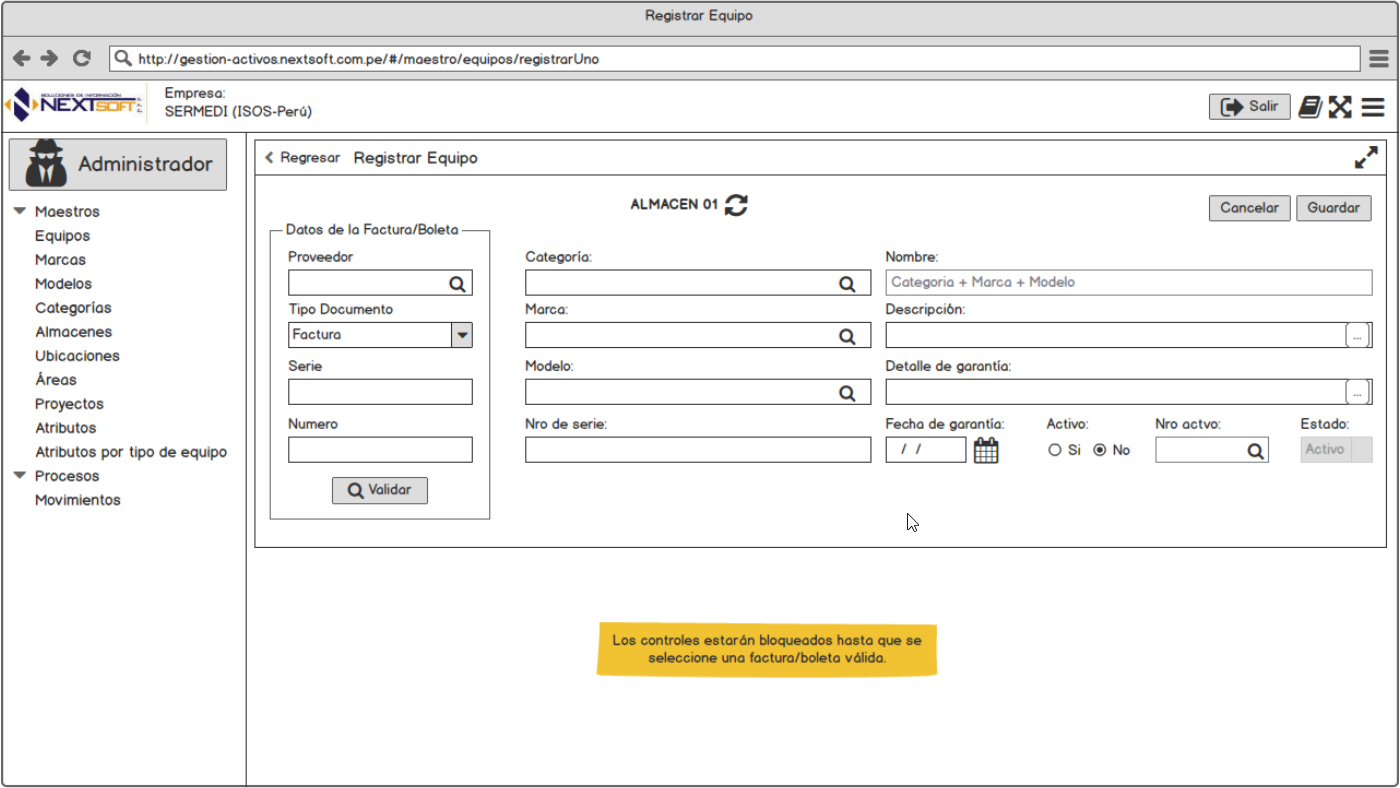
\includegraphics[width=16.5cm, angle=0]{./images/registroIndividual.png}
\end{figure}
\textbf{Pantalla de Registro Masivo de Equipos (Figura~\ref{masivo}). }La pantalla de registro masivo permite al administrador cargar un archivo Excel que contenga los detalles de m\'ultiples equipos. Esta interfaz incluye un \'area para seleccionar el archivo, una tabla con el contenido del archivo, y botones para confirmar la carga y procesamiento de los datos. Los equipos registrados a trav\'es de esta funcionalidad generar\'an movimientos de ingreso en el sistema.
\begin{figure}[H]
    \centering
    \caption{Registrar Equipos Masivamente}\label{masivo}
    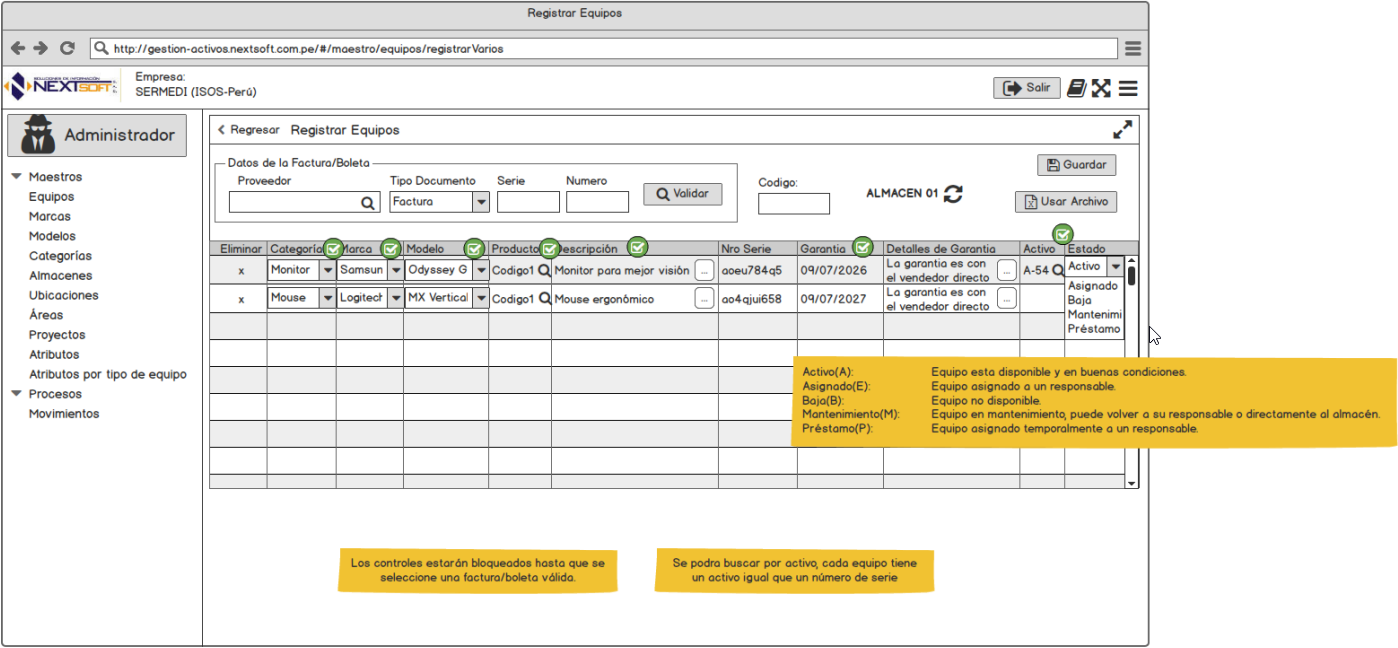
\includegraphics[width=16.5cm, angle=0]{./images/registroMasivo.png}
\end{figure}
\textbf{Pantalla de Registro de Entrega. }En la pantalla de registro de entrega, el administrador puede registrar la entrega de uno o varios equipos a un responsable. La interfaz muestra una lista de equipos disponibles y permite seleccionar aquellos que ser\'an entregados, especificando el responsable y cualquier informaci\'on adicional relevante. Una vez confirmada la entrega, los equipos seleccionados tendr\'an su estado actualizado a ``Asignado''.
\begin{figure}[H]
    \centering
    \caption{Registrar Movimiento (Primera Pesta\~{n}a)}\label{movimiento1}
    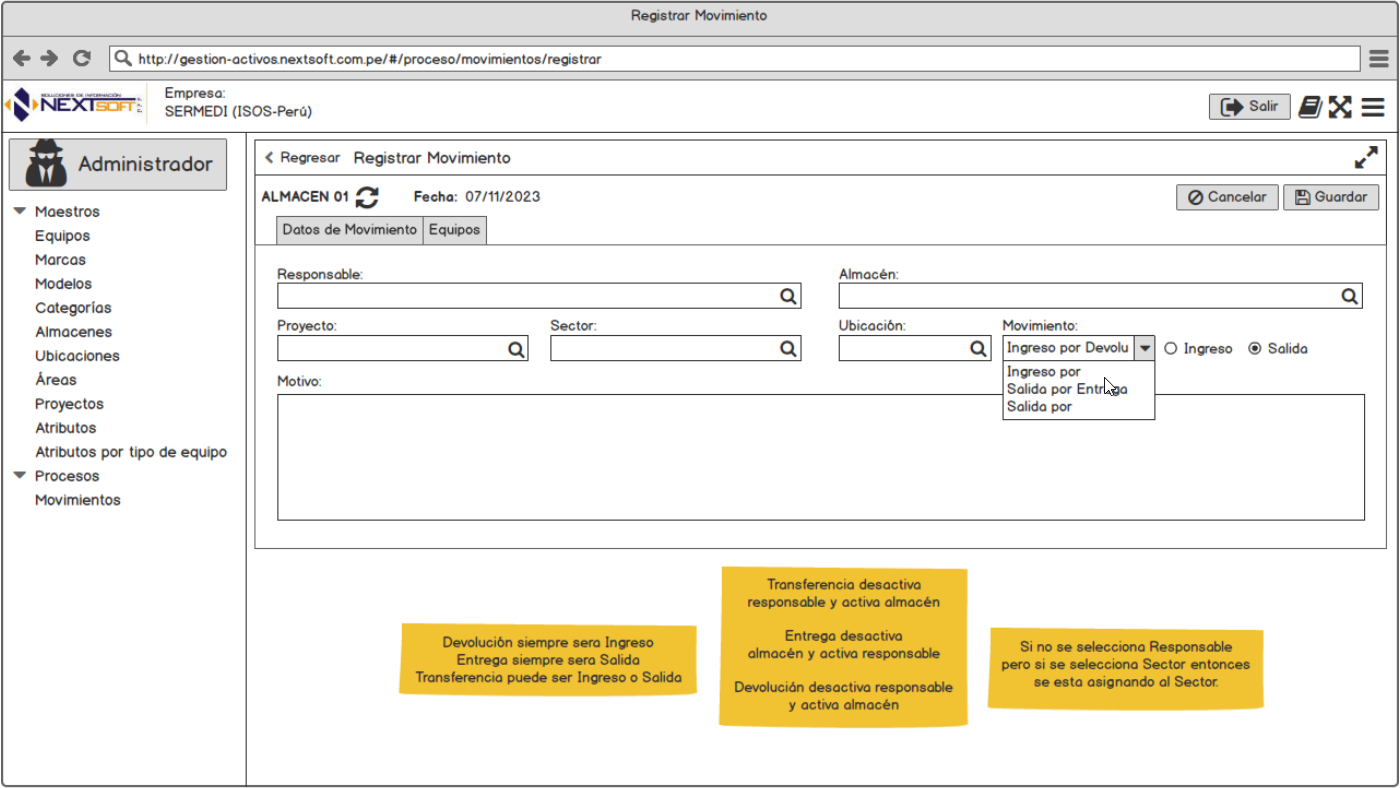
\includegraphics[width=16.5cm, angle=0]{./images/registrarMovimiento.png}
\end{figure}
\begin{figure}[H]
    \centering
    \caption{Registrar Movimiento (Segunda Pesta\~{n}a)}\label{movimiento2}
    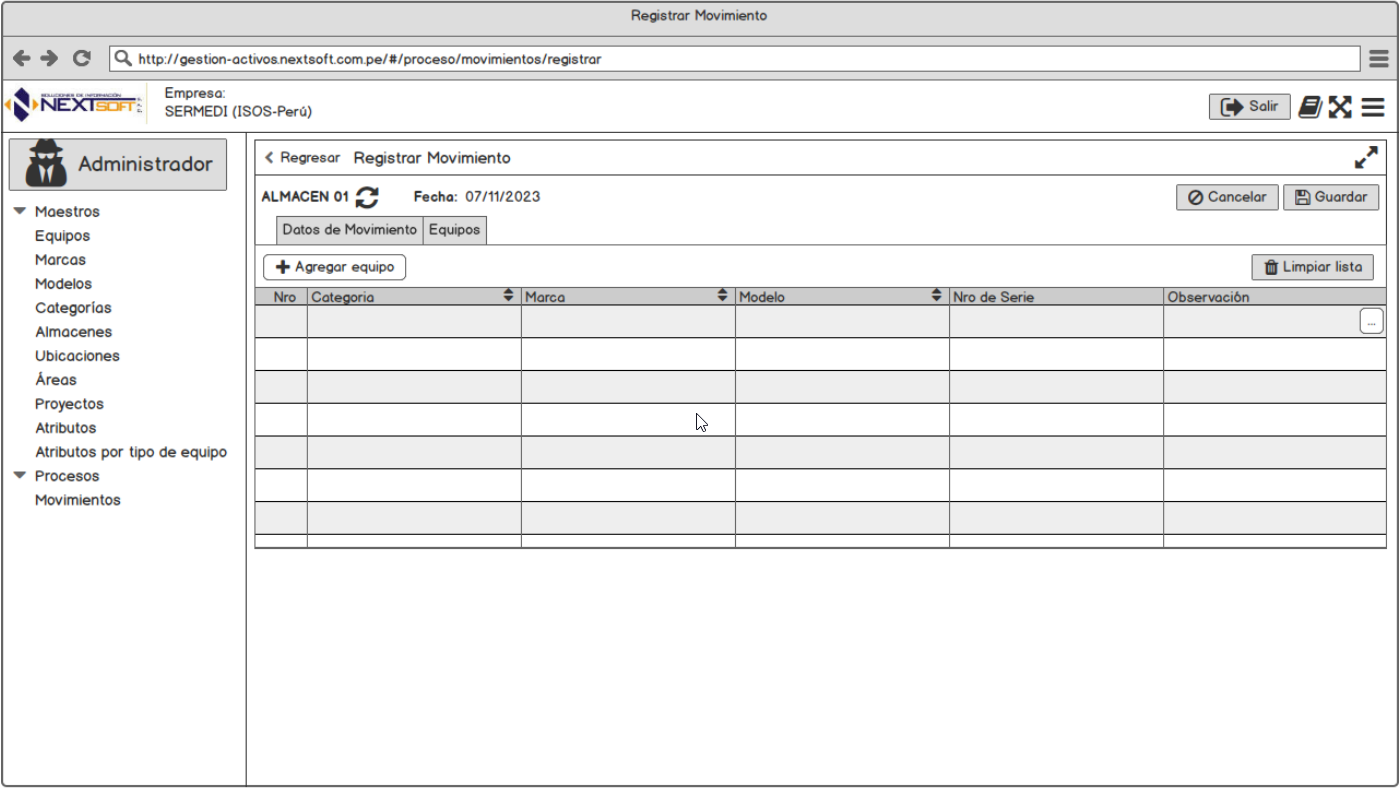
\includegraphics[width=16.5cm, angle=0]{./images/registrarMovimiento2.png}
\end{figure}
\textbf{Pantalla de Registro de Devoluci\'on. }Esta pantalla facilita el registro de la devoluci\'on de equipos al almac\'en. Similar a la pantalla de entrega, se presentan los equipos que est\'an actualmente asignados a responsables, y el administrador puede seleccionar los que se est\'an devolviendo. Al confirmar la operaci\'on, el estado de los equipos se actualiza a ``Disponible''.

\textbf{Pantalla de Registro de Transferencia. }La pantalla de registro de transferencia permite al administrador mover equipos de un almac\'en a otro. La interfaz muestra los equipos disponibles en el almac\'en de origen, y el administrador selecciona los que se transferir\'an, especificando el almac\'en de destino. Una vez completada la transferencia, se registran los movimientos correspondientes en el sistema y se actualiza la ubicaci\'on de los equipos.
\subsubsection{Arquitectura}
La arquitectura del sistema resume c\'omo las diferentes capas interact\'uan entre s\'{\i} para ofrecer una soluci\'on completa para la gesti\'on de inventario de equipos. La arquitectura est\'a dividida en tres capas principales: la Capa de Presentaci\'on, la Capa de L\'ogica de Negocio y la Capa de Acceso a Datos. Cada una de estas capas desempe\~{n}a un papel crucial en el funcionamiento del sistema, asegurando la separaci\'on de responsabilidades y facilitando el mantenimiento y la escalabilidad del m\'odulo.

\textbf{Descripci\'on de Capas. }

\textit{\textbf{Capa de Presentaci\'on (Angular 12). }}Esta capa es responsable de la interfaz de usuario (UI) y la experiencia del usuario (UX). Desarrollada en Angular 12, la Capa de Presentaci\'on maneja la interacci\'on del usuario con el sistema, permitiendo que los usuarios accedan a las funcionalidades a trav\'es de una aplicaci\'on web responsiva. Angular 12 se comunica con la Capa de L\'ogica de Negocio mediante llamadas a la API REST, enviando solicitudes y recibiendo datos para ser mostrados en la UI.

\textit{\textbf{Capa de L\'ogica de Negocio (.NET 8). }}La Capa de L\'ogica de Negocio est\'a implementada en .NET 8 y es el n\'ucleo del sistema, gestionando todas las operaciones, reglas de negocio y validaciones. Esta capa est\'a organizada en tres proyectos:
\begin{enumerate}
    \item\textbf{Service: } Este proyecto expone las funcionalidades del sistema a trav\'es de una API REST, permitiendo que la Capa de Presentaci\'on (Angular 12) interact\'ue con el sistema.
    \item\textbf{BusinessLogic: }Aqu\'{\i} se implementa la l\'ogica de negocio, donde se gestionan todas las operaciones y procesos que el sistema debe realizar, como la gesti\'on de equipos, movimientos, usuarios y configuraci\'on del sistema.
    \item\textbf{Entities: }Este proyecto contiene las entidades que representan los objetos de negocio, como Equipos, Almacenes, Movimientos, entre otros. Estas entidades son las que se manipulan en las operaciones de la l\'ogica de negocio.
\end{enumerate}

\textit{\textbf{Capa de Acceso a Datos (SQL Server). }}La Capa de Acceso a Datos se encarga de interactuar con la base de datos SQL Server. Desde la Capa de L\'ogica de Negocio, espec\'{\i}ficamente a trav\'es del proyecto BusinessLogic, se realizan las consultas y operaciones CRUD (Crear, Leer, Actualizar, Eliminar) en la base de datos. SQL Server almacena toda la informaci\'on relacionada con el inventario de equipos, incluyendo sus atributos, movimientos, estados y configuraciones.

\textbf{Patr\'on de Dise\~{n}o. }El sistema utiliza el patr\'on de dise\~{n}o MVC (Model-View-Controller) para organizar el c\'odigo y facilitar la separaci\'on de responsabilidades. En este caso, Angular 12 act\'ua como la vista (View), presentando la informaci\'on al usuario. La API REST expuesta por .NET 8 (Service) sirve como el controlador (Controller), gestionando las solicitudes del usuario y respondiendo con los datos adecuados. Finalmente, las entidades y la l\'ogica de negocio (Entities y BusinessLogic) representan el modelo (Model), donde se definen y gestionan los datos y las reglas del negocio.
\subsubsection{Desarrollo}
En la implementaci\'on del m\'odulo de gesti\'on de inventario de equipos, se adopt\'o un enfoque \'agil utilizando la metodolog\'{\i}a SCRUM, lo que permiti\'o una gesti\'on eficiente y flexible del desarrollo. A pesar de que el proyecto fue realizado por un solo desarrollador, se estructur\'o de manera que las tareas se organizaran y gestionaran de forma efectiva, similar a un entorno de desarrollo colaborativo.

\textbf{Metodolog\'{\i}a de Desarrollo. }Se utiliz\'o SCRUM como marco de trabajo para gestionar el desarrollo del m\'odulo. SCRUM, al ser una metodolog\'{\i}a \'agil, facilit\'o la adaptaci\'on continua a los cambios en los requerimientos y la retroalimentaci\'on constante. A trav\'es de la implementaci\'on de sprints cortos y enfocados, se logr\'o mantener un ritmo constante de avance, asegurando que cada incremento del producto estuviera alineado con las necesidades del proyecto.

\textbf{Fases del Proyecto. }El desarrollo se dividi\'o en 6 sprints, cada uno con una duraci\'on definida, lo que permiti\'o una entrega incremental del producto. Las fases principales incluyeron:
\begin{itemize}
    \item\textbf{Planificaci\'on: }Identificaci\'on de los requisitos del sistema y definici\'on del backlog.
    \item\textbf{Dise\~{n}o: }Creaci\'on de diagramas y dise\~{n}o de la arquitectura del sistema.
    \item\textbf{Desarrollo: }Implementaci\'on de las funcionalidades del m\'odulo, divididas en tareas manejables dentro de los sprints.
    \item\textbf{Pruebas: }Verificaci\'on de cada incremento del producto, asegurando que cumpliera con los criterios de aceptaci\'on.
    \item\textbf{Despliegue: }Integraci\'on del m\'odulo con el sistema existente y preparaci\'on para el uso en producci\'on.
\end{itemize}

\textbf{Gesti\'on de Tareas. }Las tareas del proyecto fueron organizadas y gestionadas a trav\'es de Azure DevOps. Se definieron historias de usuario para cada funcionalidad principal, y estas se dividieron en tareas individuales. A pesar de ser un solo desarrollador, el uso de herramientas de gesti\'on de proyectos como Azure DevOps permiti\'o un seguimiento detallado del progreso, la priorizaci\'on de tareas, y la resoluci\'on de problemas a medida que surg\'{\i}an.

\textbf{Colaboraci\'on y Comunicaci\'on. }Aunque no hubo un equipo de desarrollo tradicional, se utiliz\'o Subversion para la gesti\'on del c\'odigo fuente y la documentaci\'on del proyecto, garantizando que cada cambio estuviera documentado y pudiera revertirse si fuera necesario.
\newpage
\section{Desarrollo e Implementaci\'on}
\subsection{Desarrollo del M\'odulo}
El desarrollo del m\'odulo de gesti\'on de inventario de equipos fue un proceso integral que involucr\'o varias etapas t\'ecnicas, utilizando un enfoque iterativo basado en la metodolog\'{\i}a SCRUM. A continuaci\'on, se detallan los aspectos t\'ecnicos, las tecnolog\'{\i}as empleadas, y el proceso de desarrollo del m\'odulo.
\subsubsection{Tecnolog\'{\i}as Utilizadas.}
\textbf{Frontend. }El m\'odulo fue desarrollado utilizando Angular 12, un framework que permite la creaci\'on de interfaces de usuario din\'amicas, responsivas y f\'aciles de mantener. Los componentes de la interfaz de usuario se dise\~{n}aron con una l\'ogica de navegaci\'on clara y conexi\'on a la API REST del backend. Se hizo uso de servicios y m\'odulos para organizar y reutilizar el c\'odigo eficientemente.

\textbf{Backend. }Se utiliz\'o .NET 8 para implementar una API REST que interact\'ua con la base de datos y gestiona la l\'ogica de negocio. .NET 8 proporciona un entorno robusto para el desarrollo de aplicaciones empresariales, permitiendo una integraci\'on eficiente con el frontend.

\textbf{Base de Datos. }SQL Server se utiliz\'o como el sistema de gesti\'on de bases de datos para almacenar de manera segura y eficiente toda la informaci\'on relacionada con los equipos, movimientos, usuarios y configuraciones del m\'odulo. SQL Server ofrece capacidades avanzadas de manejo de datos, incluyendo transacciones, integridad referencial y consultas optimizadas.
\subsubsection{Estructura del Proyecto.}
\textbf{Capa de Presentaci\'on. }La capa de presentaci\'on se dise\~{n}\'o utilizando los principios de Angular 12, donde los componentes (C\'odigo~\ref{componente}) se organizaron en m\'odulos (C\'odigo~\ref{modulo}) para mantener la modularidad y escalabilidad de la aplicaci\'on. Los componentes de la UI se encargan de manejar la interacci\'on (C\'odigo~\ref{interaccion}) del usuario y de enviar las solicitudes al backend a trav\'es de servicios especializados (C\'odigo~\ref{conexion}). Adem\'as, se implement\'o un sistema de enrutamiento (C\'odigo~\ref{enrutamiento}) para gestionar la navegaci\'on entre las distintas vistas, y se utilizaron formularios reactivos (C\'odigo~\ref{formulario}) para capturar y validar la informaci\'on de manera eficiente.
\begin{lstlisting}[caption={M\'odulo en Angular}\label{componente}, numbers=left, breaklines=true, basicstyle=\small]
@Component({
    selector: 'ns-ss',
    templateUrl: './almacenes.component.html',
    styleUrls: ['./almacenes.component.css'],
})
export class AlmacenesComponent implements OnInit {
    public searchForm: FormGroup = new FormGroup({});
    public almacenForm: FormGroup = new FormGroup({});
    public almacenes: Almacen[] = [];
    constructor(
        private repositoryService: RepositoryService,
        private contextService: ContextService,
        private notificationService: NotificationService,
        private almacenesService: AlmacenesService
    ) { }
    ngOnInit() { }
}
\end{lstlisting}
\begin{lstlisting}[caption={M\'odulo en Angular}\label{modulo}, numbers=left, breaklines=true, basicstyle=\small]
@NgModule({
    imports: [
        AlmacenesRoutingModule,
        SharedModule,
        FeatureModule
    ],
    declarations: [AlmacenesComponent]
})
export class AlmacenesModule { }
\end{lstlisting}
\begin{lstlisting}[language=TeX, caption={M\'etodo en Componente Angular}\label{interaccion}, numbers=left, breaklines=true, basicstyle=\small]
async GuardarAlmacen() {
    if (this.isSaving) {
        return;
    }
    this.isSaving = true;
    if (!this.almacenForm.valid) {
        this.notificationService.showInformationMessage('Verifica los campos obligatorios');
        Object.keys(this.almacenForm.controls).forEach((controlName) => {
            const control = this.almacenForm.get(controlName);
            control?.markAsTouched();
        });
        this.isSaving = false;
        return;
    }
    const request: RequestRestGIV = {
        itemRequest: this.contextService.getRequest(),
        almacen: this.almacenForm.value || Almacen,
    };
    const apiresponse: ApiResponse = await this.repositoryService.AddAlmacen(request);
    if (apiresponse && apiresponse.Codigo == 0) {
        if (!request.almacen?.ALMA_CodPadre) {
            const request: RequestRestGIV = {
                itemRequest: this.contextService.getRequest(),
                almacen: this.searchForm.value as Almacen,
            };
            let ListadoAlmacenes = await this.repositoryService.GetAlmacenesPadre(request);
            this.almacenesService.SetAlmacenesPrincipal(ListadoAlmacenes);
            this.almacenes = this.almacenesService.GetAlmacenesPrincipal();
        }
        this.MView?.hide();
        this.notificationService.showSmallMessage('Se ha guardado el almacen.', true);
    }
    this.isSaving = false;
    await this.Buscar();
}
\end{lstlisting}
\begin{lstlisting}[language=TeX, caption={M\'etodo de Conexi\'on al Backend Angular}\label{conexion}, numbers=left, breaklines=true, basicstyle=\small]
public CallService = (payload: any, method: string) => new Promise<any>((resolve) =>
    this.http.post<any>((this.url + method), payload, { headers: this.core.getDefaultOptions() })
    .subscribe(
        data => resolve(data),
        err => resolve(null)
    )
)
\end{lstlisting}
\begin{lstlisting}[language=TeX, caption={Enrutamiento en Angular}\label{enrutamiento}, numbers=left, breaklines=true, basicstyle=\small]
const routes: Routes = [
    {
        path: '',
        component: MainLayoutComponent,
        canActivate: [AuthGuard],
        children: [
            {
                path: 'maestros',
                loadChildren: () => import('src/app/features/maestros/maestros.module').then((m) => m.MaestrosModule),
            },
        ],
    },
    {
        path: 'auth',
        component: AuthLayoutComponent,
        loadChildren: () => import('src/app/features/auth/auth.module').then((m) => m.AuthModule),
    },
    { path: '**', redirectTo: 'auth' },
];
@NgModule({
    imports: [RouterModule.forRoot(routes)],
    exports: [RouterModule],
})
export class AppRoutingModule { }
\end{lstlisting}
\begin{lstlisting}[language=TeX, caption={Formulario Reactivo en Angular}\label{formulario}, numbers=left, breaklines=true, basicstyle=\small]
createAlmacenForm(Mview: boolean) {
    return new FormGroup({
        ALMA_Codigo: new FormControl('', []),
        ALMA_CodPadre: new FormControl('', []),
        ALMA_Nombre: new FormControl('', [Validators.required, Validators.maxLength(100)]),
        ALMA_Descripcion: new FormControl('', [Validators.required, Validators.maxLength(100)]),
        ALMA_Estado: new FormControl(true, [Validators.required]),
    });
}
\end{lstlisting}

\textbf{Capa de L\'ogica de Negocio. }

\textit{\textbf{Service. }}Los controladores API exponen los endpoints (C\'odigo~\ref{endpoint}) necesarios para que el frontend realice operaciones CRUD (Crear, Leer, Actualizar, Eliminar) y otras interacciones con el sistema. Estos controladores gestionan las solicitudes HTTP y se comunican con el proyecto BusinessLogic para ejecutar las acciones correspondientes.
\begin{lstlisting}[language=TeX, caption={Endpoint en .NET 8}\label{endpoint}, numbers=left, breaklines=true, basicstyle=\small]
[HttpPost("AddAlmacen")]
public ActionResult<Response> AddAlmacen([FromBody] RequestRestGIV request)
{
    Response _response = new Response();
    try
    {
        int _tiempodisponible = 0;
        if (ValidarSession(request.itemRequest.SESS_Token, request.itemRequest, ref _tiempodisponible))
        {
            BLAlmacenes BL_Almacen = new BLAlmacenes();
            Almacenes almacen = new Almacenes();
            request.almacen.CopyTo(ref almacen);
            almacen.Instance = Infrastructure.Aspect.BusinessEntity.InstanceEntity.Added;
            almacen.ALMA_Estado = true;
            almacen.AUDI_UsrCrea = request.itemRequest.USER_CodUsr;
            almacen.AUDI_HostCrea = request.itemRequest.AUDI_Host;
            if (BL_Almacen.Save(ref almacen))
            {
                _response.Mensaje = $"Se realizo correctamente el registro del almacen \"{request.almacen.ALMA_Nombre}\" con el ID {almacen.ALMA_Codigo}.";
                _response.Codigo = 0;
            }
            else
            {
                _response.Codigo = 1;
                _response.Mensaje = "Ha ocurido un error al realizar el registro del almacen. </br>";
            }
            _response.TiempoSesion = _tiempodisponible;
        }
        else
        {
            _response.Codigo = 98;
            _response.Mensaje = string.Format("Mensaje: {0} - Tiempo Disponible: {1} minutos", "TOKEN No Valido", _tiempodisponible);
        }
    }
    catch (Exception ex)
    {
        String _code = Guid.NewGuid().ToString();
        _response.Codigo = 1;
        _response.Mensaje = string.Format("Error-{0}: {1}", _code, ex.Message);
        Util.WriteError(_code, ex, System.Reflection.MethodBase.GetCurrentMethod().Name);
    }
    return _response;
}
\end{lstlisting}

\textit{\textbf{BusinessLogic. }}Aqu\'{\i} se implementaron todas las reglas de negocio y validaciones necesarias para el correcto funcionamiento del m\'odulo. La l\'ogica de negocio se organiz\'o en m\'etodos y clases (C\'odigo~\ref{bl}), permitiendo una separaci\'on clara de responsabilidades. Esta capa interact\'ua directamente con la capa de acceso a datos para realizar operaciones sobre la base de datos.
\begin{lstlisting}[language=TeX, caption={M\'etodos de Business Logic en .NET 8}\label{bl}, numbers=left, breaklines=true, basicstyle=\small]
public partial class BLAlmacenes
{
    public Boolean Save(ref Almacenes Item)
    {
        try
        {
            Boolean m_isCorrect = true;
            switch (Item.Instance)
            {
                case InstanceEntity.Added:
                    m_isCorrect = Insert(ref Item); break;
                case InstanceEntity.Modified:
                    m_isCorrect = Update(ref Item); break;
                case InstanceEntity.Deleted:
                    m_isCorrect = Delete(ref Item); break;
            }
            return m_isCorrect;
        }
        catch (Exception)
        { throw; }
    }

    private bool Insert(ref Almacenes Item)
    {
        try
        {
            if (Item.Instance == InstanceEntity.Added)
            {
                SqlCommand DASqlCommand = DataAccessEnterpriseSQL.DAAsignarProcedure("GIV_ALMASI_UnReg");
                DataAccessEnterpriseSQL.DAAgregarParametro(DASqlCommand, "@ALMA_Codigo", Item.ALMA_Codigo, SqlDbType.VarChar, 6, ParameterDirection.InputOutput);
                DataAccessEnterpriseSQL.DAAgregarParametro(DASqlCommand, "@ALMA_CodPadre", string.IsNullOrEmpty(Item.ALMA_CodPadre) ? null : Item.ALMA_CodPadre, SqlDbType.VarChar, 6, ParameterDirection.Input);
                DataAccessEnterpriseSQL.DAAgregarParametro(DASqlCommand, "@ALMA_Nombre", Item.ALMA_Nombre, SqlDbType.VarChar, 100, ParameterDirection.Input);
                DataAccessEnterpriseSQL.DAAgregarParametro(DASqlCommand, "@ALMA_Descripcion", Item.ALMA_Descripcion, SqlDbType.VarChar, 100, ParameterDirection.Input);
                DataAccessEnterpriseSQL.DAAgregarParametro(DASqlCommand, "@ALMA_Estado", Item.ALMA_Estado, SqlDbType.Bit, 1, ParameterDirection.Input);
                DataAccessEnterpriseSQL.DAAgregarParametro(DASqlCommand, "@AUDI_UsrCrea", Item.AUDI_UsrCrea, SqlDbType.VarChar, 20, ParameterDirection.Input);
                DataAccessEnterpriseSQL.DAAgregarParametro(DASqlCommand, "@AUDI_HostCrea", Item.AUDI_HostCrea, SqlDbType.VarChar, 50, ParameterDirection.Input);
                if (DataAccessEnterpriseSQL.DAExecuteNonQuery(DASqlCommand, null) > 0)
                {
                    if (DASqlCommand.Parameters["@ALMA_Codigo"].Value != DBNull.Value && !String.IsNullOrEmpty(DASqlCommand.Parameters["@ALMA_Codigo"].Value.ToString()))
                    { Item.ALMA_Codigo = DASqlCommand.Parameters["@ALMA_Codigo"].Value.ToString(); }
                    return true;
                }
                else
                { return false; }
            }
            else
            { return true; }
        }
        catch (Exception)
        { throw; }
    }
}
\end{lstlisting}

\textit{\textbf{Entities. }}Las entidades (C\'odigo~\ref{entidad}) representan los datos clave dentro del sistema, como equipos, categor\'{\i}as, movimientos, y usuarios. Estas entidades est\'an definidas con sus respectivas relaciones, lo que permite una representaci\'on clara y estructurada de la informaci\'on en la base de datos.
\begin{lstlisting}[language=TeX, caption={Entidad en .NET 8}\label{entidad}, numbers=left, breaklines=true, basicstyle=\small]
public partial class Almacenes
{
    #region [ Variables ]
    private String m_alma_codigo;
    private String m_alma_codpadre;
    private String m_alma_nombre;
    private String m_alma_descripcion;
    private Nullable<Boolean> m_alma_estado;
    private String m_audi_usrcrea;
    private Nullable<DateTime> m_audi_feccrea;
    private String m_audi_hostcrea;
    private String m_audi_usrmod;
    private Nullable<DateTime> m_audi_fecmod;
    private String m_audi_hostmod;
    #endregion
    #region [ Constructores ]
    public Almacenes(){ }
    #endregion
    #region [ Propiedades ]
    [DataMember]
    public String ALMA_Codigo
    {
        get { return m_alma_codigo; }
        set
        {
            if (m_alma_codigo != value)
            {
                m_alma_codigo = value;
                OnPropertyChanged("ALMA_Codigo");
            }
        }
    }
    [DataMember]
    public String ALMA_CodPadre
    {
        get { return m_alma_codpadre; }
        set
        {
            if (m_alma_codpadre != value)
            {
                m_alma_codpadre = value;
                OnPropertyChanged("ALMA_CodPadre");
            }
        }
    }
    [DataMember]
    public String ALMA_Nombre
    {
        get { return m_alma_nombre; }
        set
        {
            if (m_alma_nombre != value)
            {
                m_alma_nombre = value;
                OnPropertyChanged("ALMA_Nombre");
            }
        }
    }
    [DataMember]
    public String ALMA_Descripcion
    {
        get { return m_alma_descripcion; }
        set
        {
            if (m_alma_descripcion != value)
            {
                m_alma_descripcion = value;
                OnPropertyChanged("ALMA_Descripcion");
            }
        }
    }
    [DataMember]
    public Nullable<Boolean> ALMA_Estado
    {
        get { return m_alma_estado; }
        set
        {
            if (m_alma_estado != value)
            {
                m_alma_estado = value;
                OnPropertyChanged("ALMA_Estado");
            }
        }
    }
    [IgnoreDataMember]
    public String AUDI_UsrCrea
    {
        get { return m_audi_usrcrea; }
        set
        {
            if (m_audi_usrcrea != value)
            {
                m_audi_usrcrea = value;
                OnPropertyChanged("AUDI_UsrCrea");
            }
        }
    }
    [IgnoreDataMember]
    [DisplayFormat(DataFormatString = "{0:yyyy-MM-dd}", ApplyFormatInEditMode = true)]
    public Nullable<DateTime> AUDI_FecCrea
    {
        get { return m_audi_feccrea; }
        set
        {
            if (m_audi_feccrea != value)
            {
                m_audi_feccrea = value;
                OnPropertyChanged("AUDI_FecCrea");
            }
        }
    }
    [IgnoreDataMember]
    public String AUDI_HostCrea
    {
        get { return m_audi_hostcrea; }
        set
        {
            if (m_audi_hostcrea != value)
            {
                m_audi_hostcrea = value;
                OnPropertyChanged("AUDI_HostCrea");
            }
        }
    }
    [IgnoreDataMember]
    public String AUDI_UsrMod
    {
        get { return m_audi_usrmod; }
        set
        {
            if (m_audi_usrmod != value)
            {
                m_audi_usrmod = value;
                OnPropertyChanged("AUDI_UsrMod");
            }
        }
    }
    [IgnoreDataMember]
    [DisplayFormat(DataFormatString = "{0:yyyy-MM-dd}", ApplyFormatInEditMode = true)]
    public Nullable<DateTime> AUDI_FecMod
    {
        get { return m_audi_fecmod; }
        set
        {
            if (m_audi_fecmod != value)
            {
                m_audi_fecmod = value;
                OnPropertyChanged("AUDI_FecMod");
            }
        }
    }
    [IgnoreDataMember]
    public String AUDI_HostMod
    {
        get { return m_audi_hostmod; }
        set
        {
            if (m_audi_hostmod != value)
            {
                m_audi_hostmod = value;
                OnPropertyChanged("AUDI_HostMod");
            }
        }
    }
    #endregion
    #region [ CopyTo ]
    public void CopyTo(ref Almacenes Item)
    {
        try
        {
            if (Item == null) { Item = new Almacenes(); }
            Item.ALMA_Codigo = this.ALMA_Codigo;
            Item.ALMA_CodPadre = this.ALMA_CodPadre;
            Item.ALMA_Nombre = this.ALMA_Nombre;
            Item.ALMA_Descripcion = this.ALMA_Descripcion;
            Item.ALMA_Estado = this.ALMA_Estado;
            Item.AUDI_HostCrea = this.AUDI_HostCrea;
            Item.AUDI_HostMod = this.AUDI_HostMod;
            Item.ALMA_NomPadre = this.ALMA_NomPadre;
        }
        catch (Exception ex)
        { throw ex; }
    }
    #endregion
}
\end{lstlisting}

\textbf{Capa de Acceso a Datos. }La capa de acceso a datos se implement\'o en el proyecto BusinessLogic, utilizando procedimientos almacenados (C\'odigo~\ref{sp}) para ejecutar consultas a la base de datos. Esto permiti\'o una interacci\'on eficiente y segura con SQL Server, manteniendo la l\'ogica de acceso a datos separada de la l\'ogica de negocio.
\begin{lstlisting}[language=TeX, caption={Procedimiento Almacenado en SQL Server}\label{sp}, numbers=left, breaklines=true, basicstyle=\small]
CREATE PROCEDURE dbo.GIV_ALMASI_UnReg 
    @ALMA_Codigo      VARCHAR(6) OUTPUT
  , @ALMA_CodPadre    VARCHAR(6)
  , @ALMA_Nombre      VARCHAR(100)
  , @ALMA_Descripcion VARCHAR(100)
  , @ALMA_Estado      BIT
  , @AUDI_UsrCrea     VARCHAR(20)
  , @AUDI_HostCrea    VARCHAR(50)  
AS  
BEGIN
    IF((SELECT ALMA_CodPadre 
          FROM GIV_Almacenes  
         WHERE ALMA_Codigo = @ALMA_CodPadre) IS NULL)  
        BEGIN  
            SET @ALMA_Codigo = ISNULL((SELECT MAX(CONVERT(INT,ALMA_Codigo))  
                                         FROM GIV_Almacenes), 0) + 1
            INSERT INTO GIV_Almacenes  
            ( ALMA_Codigo , ALMA_CodPadre , ALMA_Nombre , ALMA_Descripcion     
            , ALMA_Estado , AUDI_UsrCrea  , AUDI_FecCrea, AUDI_HostCrea    )  
            VALUES  
            ( @ALMA_Codigo, @ALMA_CodPadre, @ALMA_Nombre, @ALMA_Descripcion     
            , @ALMA_Estado, @AUDI_UsrCrea , GETDATE()   , @AUDI_HostCrea   )  
        END
    ELSE  
        BEGIN  
            RAISERROR('El almacen superior elegido no es valido, seleccione otro para continuar.', 18, 1)  
            RETURN  
        END  
END
\end{lstlisting}
\subsubsection{Proceso de Desarrollo.}
\textbf{Metodolog\'{\i}a de Desarrollo. }El proyecto fue gestionado utilizando la metodolog\'{\i}a \'agil SCRUM, lo que permiti\'o un desarrollo iterativo y adaptable. A lo largo de los seis sprints, se realiz\'o un seguimiento continuo del progreso y se ajustaron las tareas seg\'un las necesidades emergentes. La gesti\'on de tareas y sprints se llev\'o a cabo en Azure DevOps y la versi\'on del c\'odigo fue controlada mediante Subversion, asegurando un historial claro de cambios y la capacidad de revertir a versiones anteriores si era necesario.

\textbf{Desarrollo Iterativo. }El m\'odulo se desarroll\'o en seis sprints, cada uno con un objetivo claro y espec\'{\i}fico:
\begin{enumerate}
    \item\textbf{An\'alisis y dise\~{n}o: }Se realiz\'o el an\'alisis de requerimientos y el dise\~{n}o de mockups.
    \item\textbf{Desarrollo de mantenimiento de maestros: }Implementaci\'on de funcionalidades para la gesti\'on de datos maestros.
    \item\textbf{Desarrollo de registro de equipos: }Creaci\'on de las funcionalidades para registrar equipos de manera individual y masiva.
    \item\textbf{Desarrollo de registro de movimientos: }Implementaci\'on de funcionalidades para registrar entregas, devoluciones y transferencias de equipos.
    \item\textbf{Desarrollo de reportes: }Creaci\'on de reportes detallados sobre equipos y movimientos.
    \item\textbf{Despliegue del m\'odulo: }Despliegue final del m\'odulo y preparaci\'on para su uso en el entorno de producci\'on.
\end{enumerate}

\textbf{Pruebas Realizadas. }Las pruebas se realizaron en diferentes niveles para asegurar la calidad y funcionalidad del m\'odulo:
\begin{itemize}
    \item\textbf{Pruebas de usuario: }Se llevaron a cabo pruebas de usuario para validar que el m\'odulo cumpliera con los requerimientos y expectativas.
    \item\textbf{Pruebas del backend: }Utilizando Postman, se probaron exhaustivamente las APIs, verificando que respondieran correctamente y cumplieran con las especificaciones.
    \item\textbf{Pruebas del frontend: }Se realizaron pruebas en los formularios reactivos de Angular para asegurar que validaran correctamente la informaci\'on obligatoria. Adem\'as, se prob\'o la interacci\'on entre el frontend y el backend.
    \item\textbf{Pruebas de integraci\'on: }Se verific\'o que la comunicaci\'on entre el frontend y el backend funcionara sin problemas, incluyendo pruebas de guardado y recuperaci\'on de datos desde la base de datos.
    \item\textbf{Pruebas de guardado y recuperaci\'on de la base de datos: }Se llevaron a cabo pruebas para asegurar que los datos se guardaran y recuperaran correctamente en SQL Server, garantizando la integridad y consistencia de la informaci\'on almacenada.
\end{itemize}
\subsection{Integraci\'on con Otros Sistemas}
\subsubsection{Integraci\'on con el ERP de NextSoft}
\textbf{Autenticaci\'on. }El m\'odulo utiliza el sistema NextSis para gestionar el inicio de sesi\'on. Las credenciales del ERP de NextSoft, proporcionadas a trav\'es de NextSis, permiten que solo usuarios autorizados accedan al m\'odulo. Esta integraci\'on asegura que el acceso al sistema est\'e restringido y que se mantenga la coherencia en la gesti\'on de usuarios a trav\'es de los diferentes sistemas del ERP.

\textbf{Sincronizaci\'on de Datos. }El m\'odulo de gesti\'on de inventario de equipos est\'a dise\~{n}ado para integrarse con varios sistemas del ERP. Esto incluye:
\begin{itemize}
    \item\textbf{Sistema de log\'{\i}stica: }Se sincroniza con el sistema de log\'{\i}stica para utilizar datos de marcas y productos. Esto garantiza que la informaci\'on sobre los equipos sea precisa y est\'e alineada con las categor\'{\i}as y especificaciones definidas en el sistema de log\'{\i}stica.
    \item\textbf{Sistema de activos: }Se conecta con el sistema de activos para obtener y relacionar datos de activos existentes. Esta integraci\'on permite una gesti\'on m\'as eficiente al asociar los datos de los activos con los equipos registrados en el m\'odulo.
    \item\textbf{Sistema de tesorer\'{\i}a: }El m\'odulo se integra con el sistema de tesorer\'{\i}a para acceder a comprobantes de compra, como boletas y facturas. Esto facilita la correcta asociaci\'on de los equipos con sus documentos de adquisici\'on, asegurando que la informaci\'on financiera y de inventario est\'e correctamente vinculada.
\end{itemize}
\subsubsection{Beneficios de la Integraci\'on}
\begin{itemize}
    \item\textbf{Optimizaci\'on de procesos: }La integraci\'on con los sistemas de log\'{\i}stica, activos, y tesorer\'{\i}a facilita la automatizaci\'on de procesos y reduce la duplicaci\'on de datos. Al sincronizar la informaci\'on entre los sistemas, se minimiza la necesidad de ingresar datos manualmente y se asegura que la informaci\'on est\'e actualizada en tiempo real. Esto contribuye a una gesti\'on de inventario m\'as eficiente y a una reducci\'on de errores.
    \item\textbf{Mejora en la Toma de Decisiones: }La integraci\'on permite una visi\'on m\'as completa y precisa de la informaci\'on relacionada con el inventario de equipos. Al tener acceso a datos consolidados de los sistemas de log\'{\i}stica, activos y tesorer\'{\i}a, los usuarios pueden tomar decisiones m\'as informadas basadas en informaci\'on actualizada y relevante. Esto facilita la planificaci\'on, el control y la toma de decisiones estrat\'egicas relacionadas con el manejo de inventarios.
\end{itemize}
\newpage
\section{Resultados}
En esta secci\'on se presentan los resultados obtenidos tras la implementaci\'on del m\'odulo de gesti\'on de inventario de equipos. Se describen los aspectos m\'as destacados del sistema, incluyendo su funcionamiento, interfaces desarrolladas, generaci\'on de reportes, y la integraci\'on con otros sistemas dentro de la empresa.
\subsection{Implementaci\'on del Sistema}
A trav\'es de la API REST implementada en~.NET 8, el sistema permite una comunicaci\'on fluida y eficiente, asegurando un manejo robusto de la l\'ogica de negocio y acceso a los datos almacenados en SQL Server. La integraci\'on con el ERP de NextSoft mediante el sistema NextSis garantiza que la autenticaci\'on y autorizaci\'on de los usuarios se gestionen de manera centralizada y segura.
\subsection{Interfaces Desarrolladas}
\subsubsection{Pantalla de Inicio de Sesi\'on}
La pantalla de inicio de sesi\'on [Figura~\ref{loginProd}] permite a los usuarios acceder al m\'odulo utilizando sus credenciales del ERP de NextSoft, gestionadas a trav\'es de NextSis. La autenticaci\'on centralizada asegura que solo los usuarios autorizados puedan acceder al sistema, manteniendo la seguridad y el control de acceso.
\begin{figure}[H]
    \centering
    \caption{Pantalla de Inicio de Sesi\'on}\label{loginProd}
    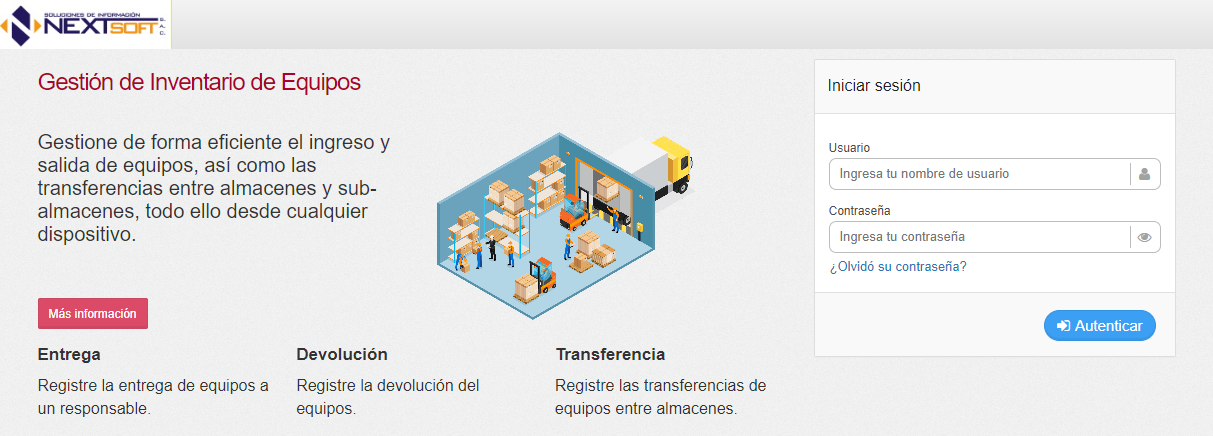
\includegraphics[width=16.5cm]{./images/loginProd.png}
\end{figure}
\subsubsection{Pantalla de Registro Individual de Equipo}
La interfaz para el registro individual de equipos [Figura~\ref{datosEquipo}] permite a los administradores ingresar detalladamente la informaci\'on de cada equipo, asi como sus atributos [Figura~\ref{atributosEquipo}] y sus calibraciones [Figura~\ref{calibracionesEquipo}], asegurando que cada registro est\'e completo.
\begin{figure}[H]
    \centering
    \caption{Pantalla de Registro Individual de Equipo (Informaci\'on)}\label{datosEquipo}
    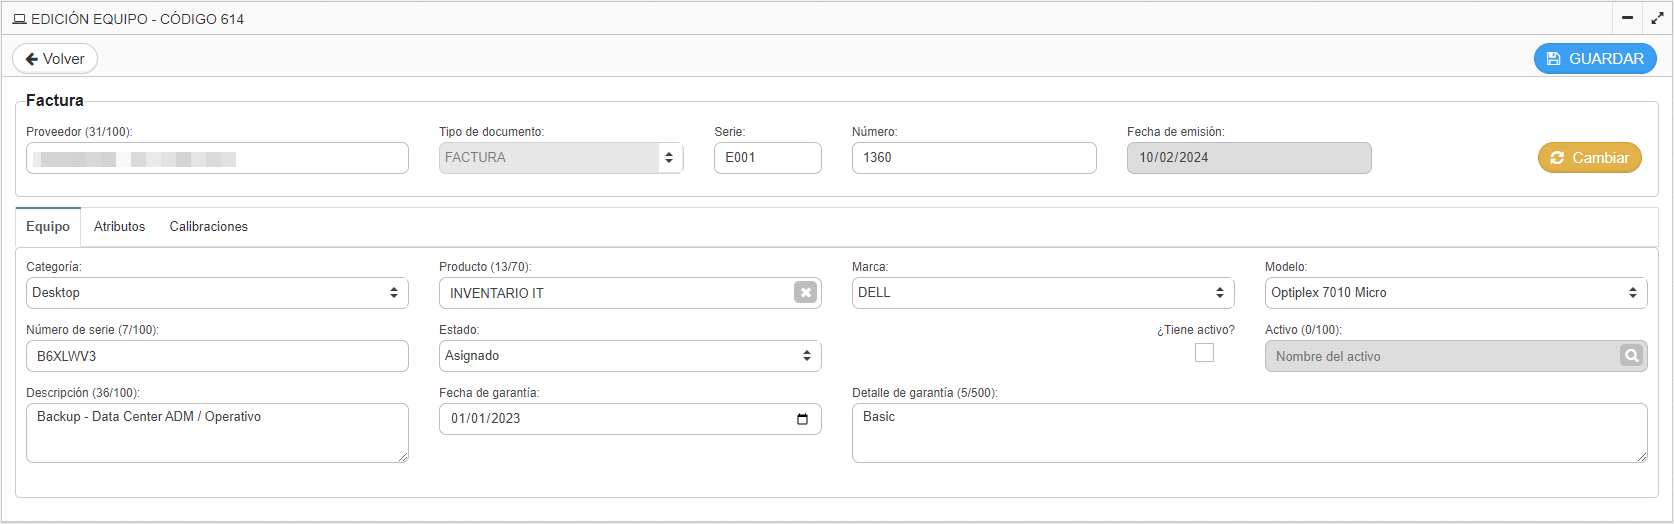
\includegraphics[width=16.5cm]{./images/datosEquipo.png}
\end{figure}
\begin{figure}[H]
    \centering
    \caption{Pantalla de Registro Individual de Equipo (Atributos)}\label{atributosEquipo}
    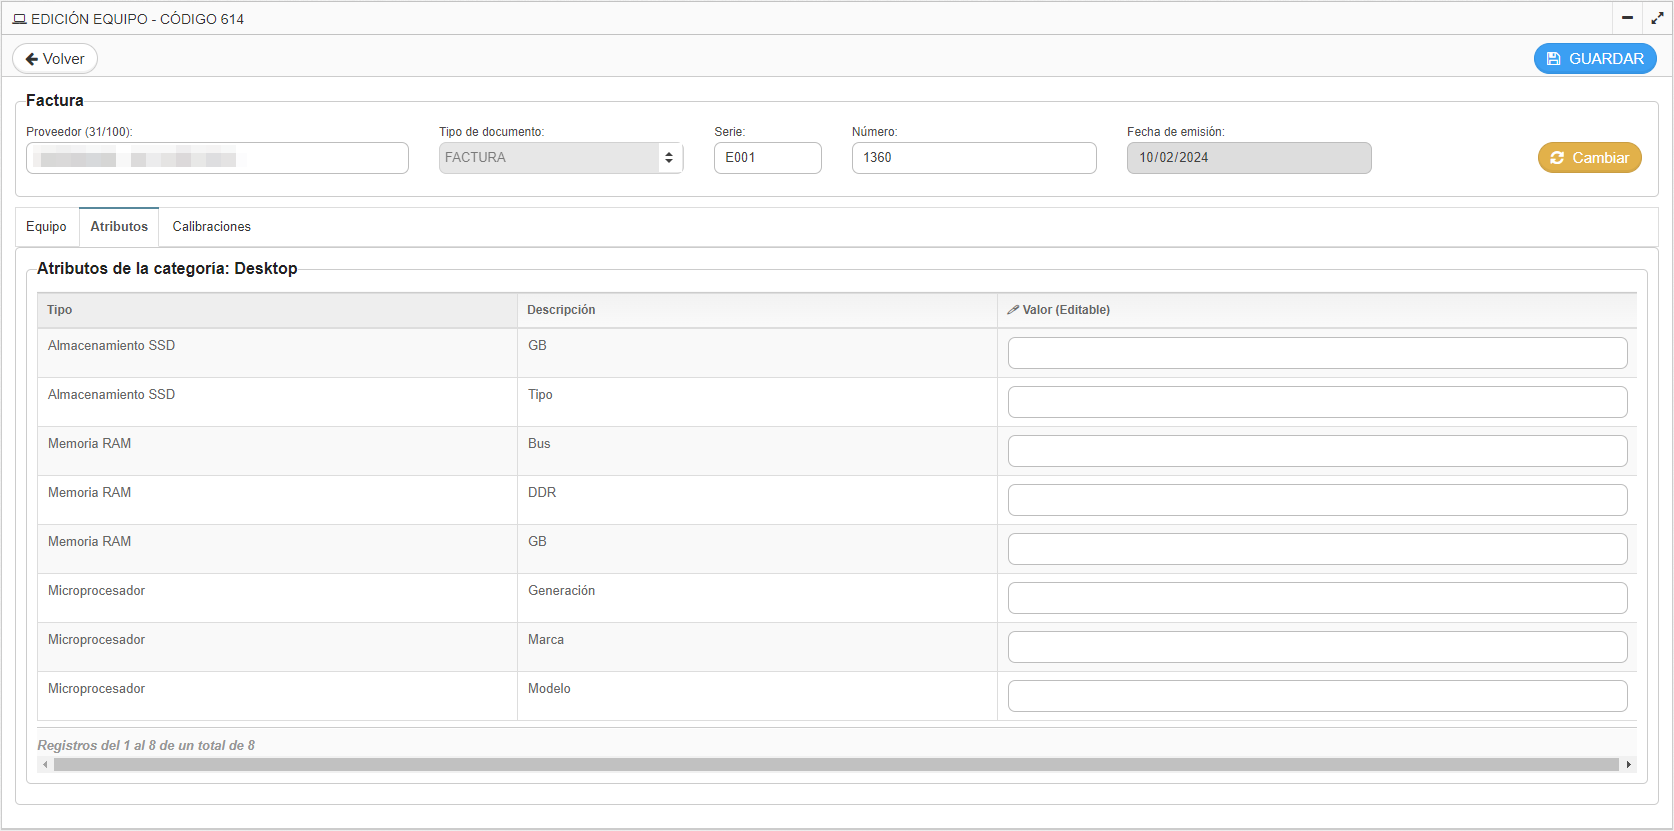
\includegraphics[width=16.5cm]{./images/equipoAtributos.png}
\end{figure}
\begin{figure}[H]
    \centering
    \caption{Pantalla de Registro Individual de Equipo (Calibraciones)}\label{calibracionesEquipo}
    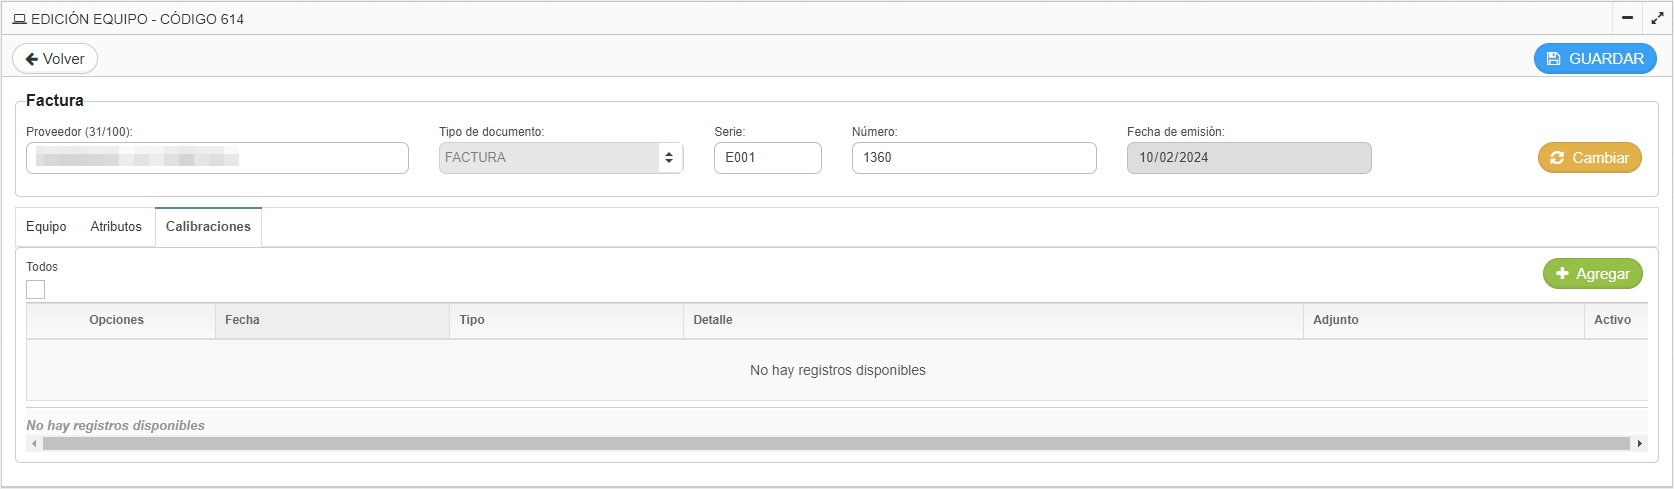
\includegraphics[width=16.5cm]{./images/calibracionesEquipo.png}
\end{figure}
\subsubsection{Pantalla de Registro Masivo de Equipos}
Para facilitar la carga de m\'ultiples equipos, se desarroll\'o una interfaz para el registro masivo [Figura~\ref{equipoMasivo}], que permite al administrador cargar un archivo Excel con los datos de los equipos. Esta funcionalidad agiliza el proceso de registro y minimiza el riesgo de errores en la entrada de datos.
\begin{figure}[H]
    \centering
    \caption{Pantalla de Registro Masivo de Equipos}\label{equipoMasivo}
    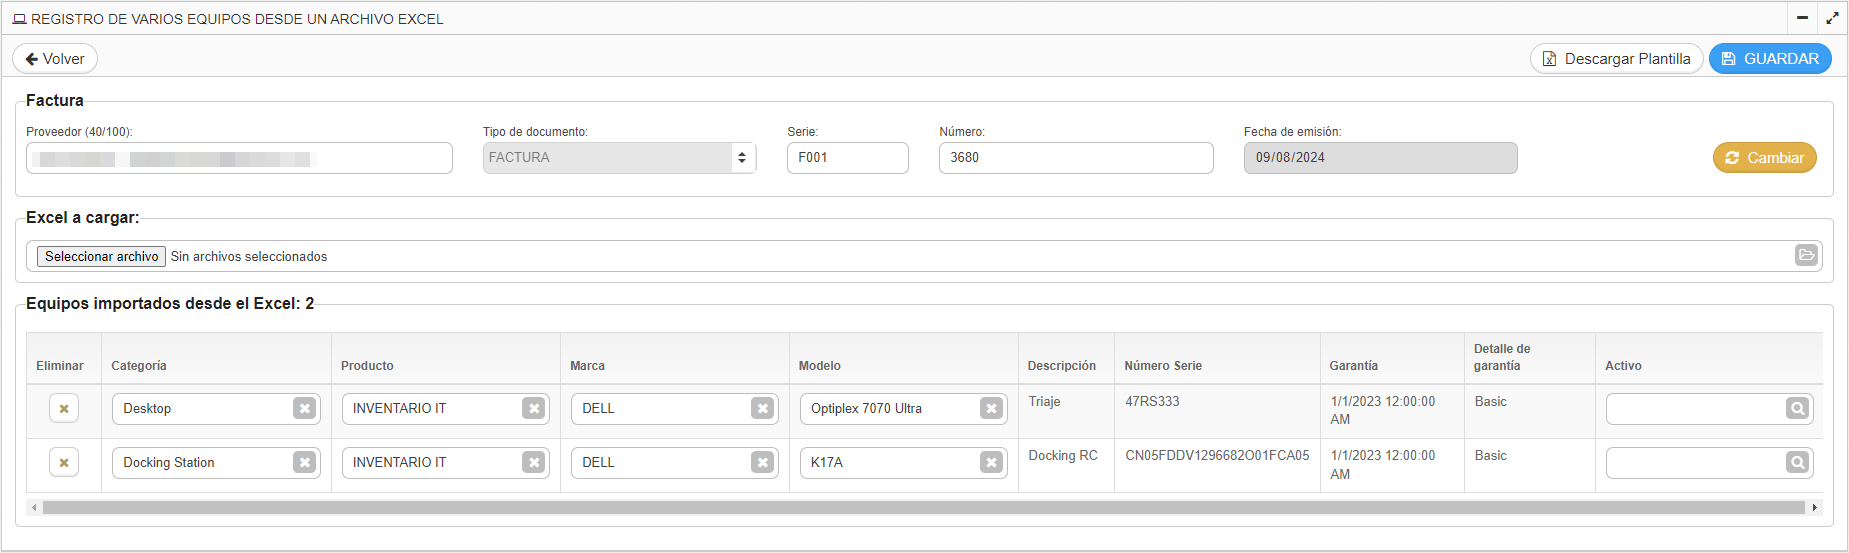
\includegraphics[width=16.5cm]{./images/equipoMasivo.png}
\end{figure}
\subsubsection{Pantalla de Registro de Entregas}
La interfaz de registro de entregas [Figura~\ref{entrega}] permite a los administradores documentar la entrega de equipos a los responsables correspondientes. El estado de los equipos se actualiza autom\'aticamente a "Asignado", garantizando que la informaci\'on en el sistema est\'e siempre actualizada.
\begin{figure}[H]
    \centering
    \caption{Pantalla de Registro de Entrega}\label{entrega}
    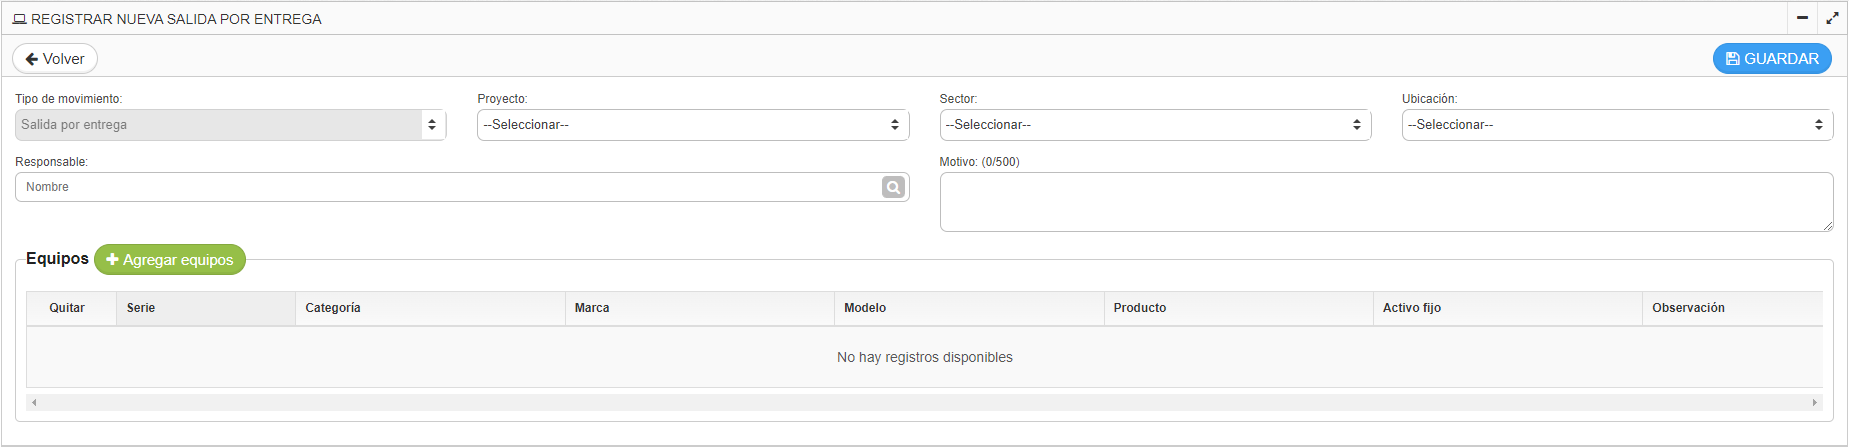
\includegraphics[width=16.5cm]{./images/entregaEquipo.png}
\end{figure}
\subsubsection{Pantalla de Registro de Devoluciones}
Similar a la entrega, la pantalla de registro de devoluciones [Figura~\ref{devolucion}] facilita la documentaci\'on de equipos que han sido devueltos al almac\'en, actualizando su estado a ``Disponible''.
\begin{figure}[H]
    \centering
    \caption{Pantalla de Registro de Devoluci\'on}\label{devolucion}
    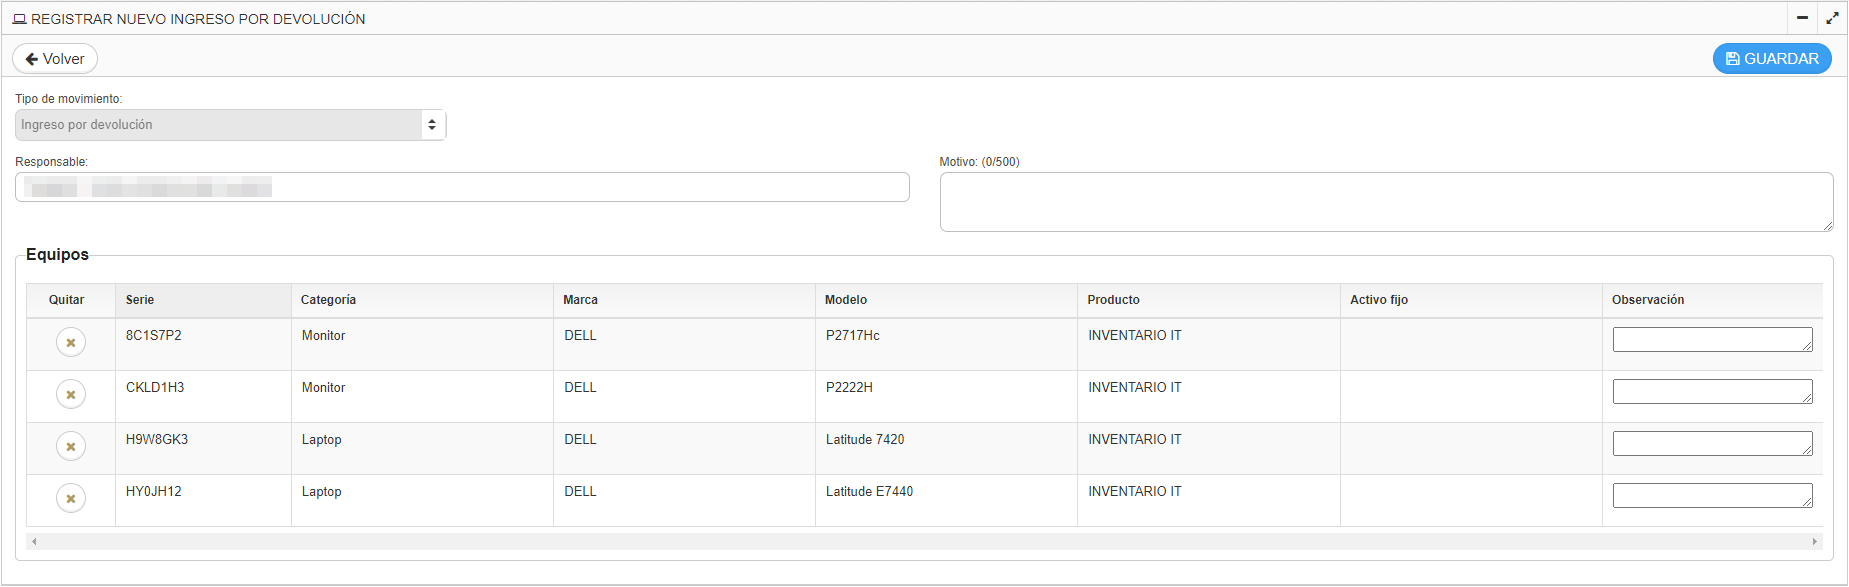
\includegraphics[width=16.5cm]{./images/devolucionEquipo.png}
\end{figure}
\subsubsection{Pantalla de Registro de Transferencias}
La pantalla para registrar transferencias [Figura~\ref{transferencia}] permite mover equipos de un almac\'en a otro, generando los movimientos necesarios y asegurando que el inventario se mantenga preciso y sincronizado entre las diferentes ubicaciones.
\begin{figure}[H]
    \centering
    \caption{Pantalla de Registro de Transferencia}\label{transferencia}
    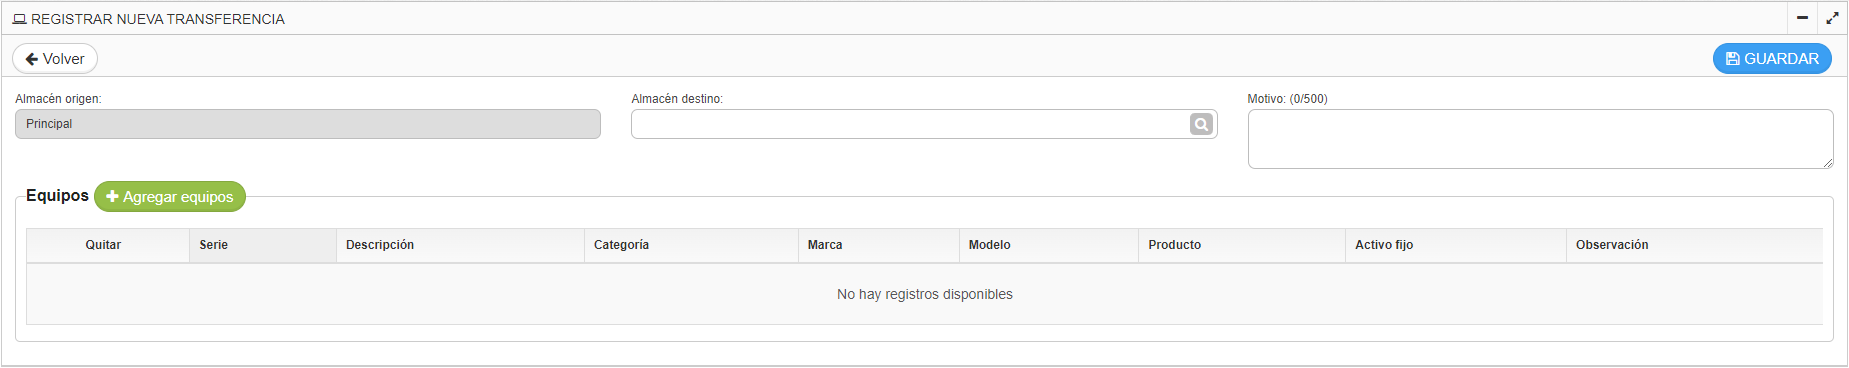
\includegraphics[width=16.5cm]{./images/transferencia.png}
\end{figure}
\subsection{Generaci\'on de Reportes}
El m\'odulo cuenta con una funcionalidad avanzada de generaci\'on de reportes [Figura~\ref{reportes}] que permite a los usuarios crear informes detallados y personalizables sobre el inventario de equipos. Estos reportes pueden filtrarse por m\'ultiples criterios, como estado, categor\'{\i}a, almac\'en, y otros par\'ametros relevantes, proporcionando una visi\'on integral y precisa del inventario. Adem\'as de los reportes generales, cada movimiento realizado en el sistema (como entregas, devoluciones y transferencias) genera un reporte espec\'{\i}fico, como cargos de entrega [Figura~\ref{cargoEntrega}], cargos de devoluci\'on [Figura~\ref{cargoDevolucion}] y cargos de transferencia [Figura~\ref{cargoTransferencia}]. Estos documentos facilitan el seguimiento y la documentaci\'on de cada operaci\'on. Los reportes pueden ser exportados en formatos como Excel, lo que permite un an\'alisis detallado y la f\'acil presentaci\'on de la informaci\'on.
\begin{figure}[H]
    \centering
    \caption{Reportes}\label{reportes}
    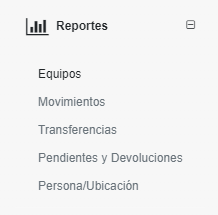
\includegraphics[scale=1]{./images/reportes.png}
\end{figure}
\begin{figure}[h]
    \caption{Cargos de Movimientos}\label{cargos}
    \centering
    \begin{subfigure}[b]{0.3\textwidth}
        \centering
        \caption{Cargo de Entrega}\label{cargoEntrega}
        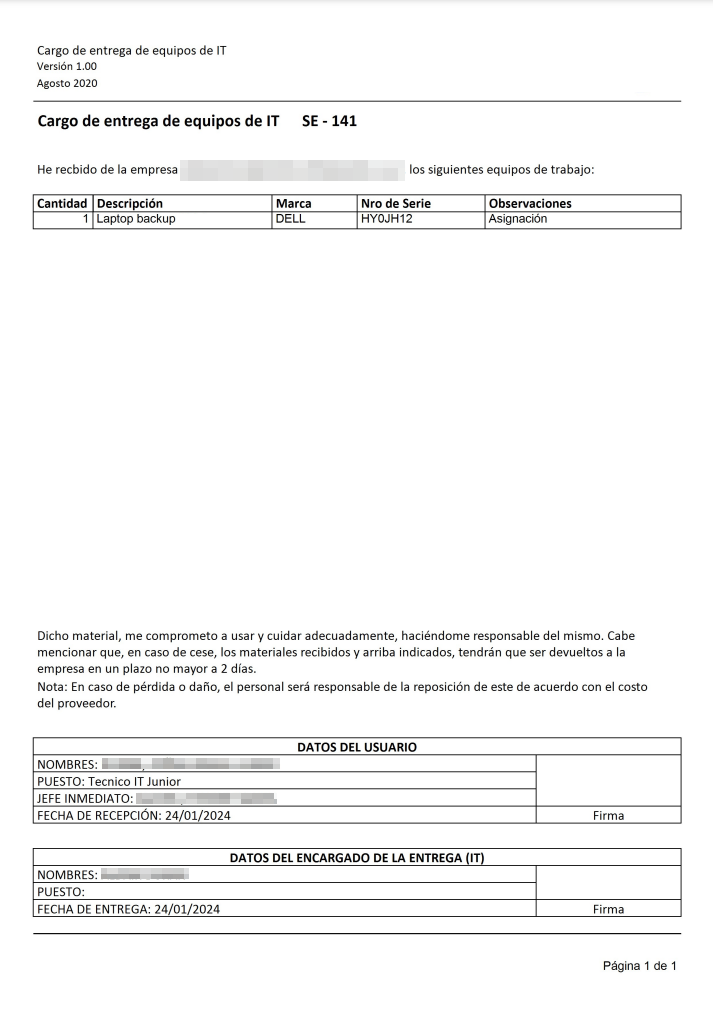
\includegraphics[width=\textwidth]{./images/reporteEntrega.png}
    \end{subfigure}
    \hfill
    \begin{subfigure}[b]{0.3\textwidth}
        \centering
        \caption{Cargo de Devoluci\'on}\label{cargoDevolucion}
        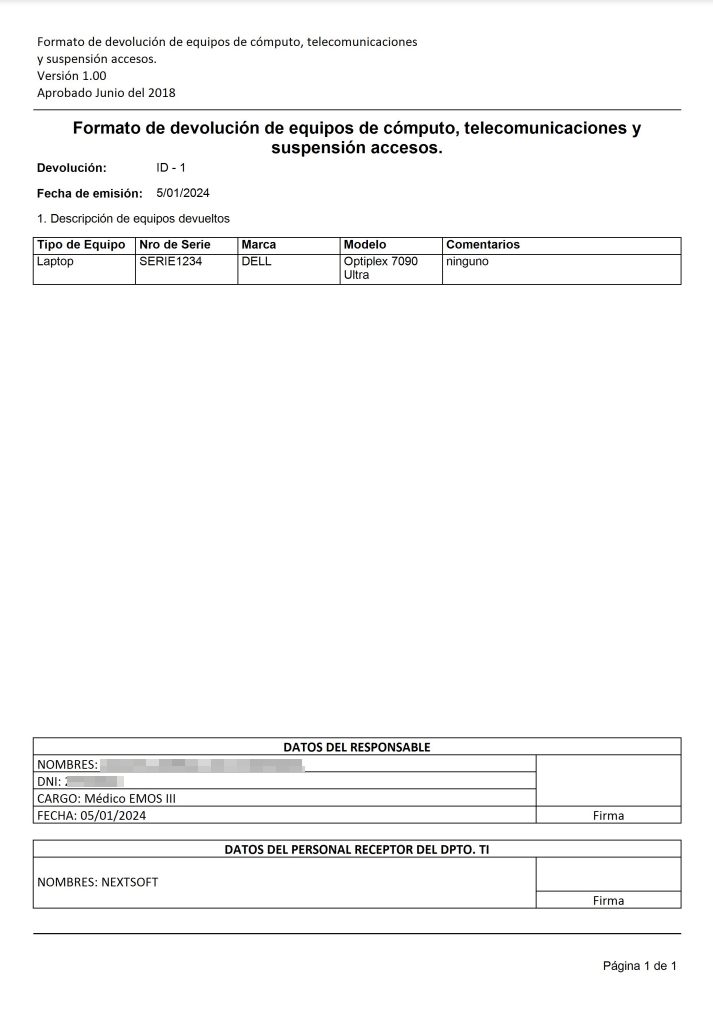
\includegraphics[width=\textwidth]{./images/reporteDevolucion.png}
    \end{subfigure}
    \hfill
    \begin{subfigure}[b]{0.3\textwidth}
        \centering
        \caption{Cargo de Transferencia}\label{cargoTransferencia}
        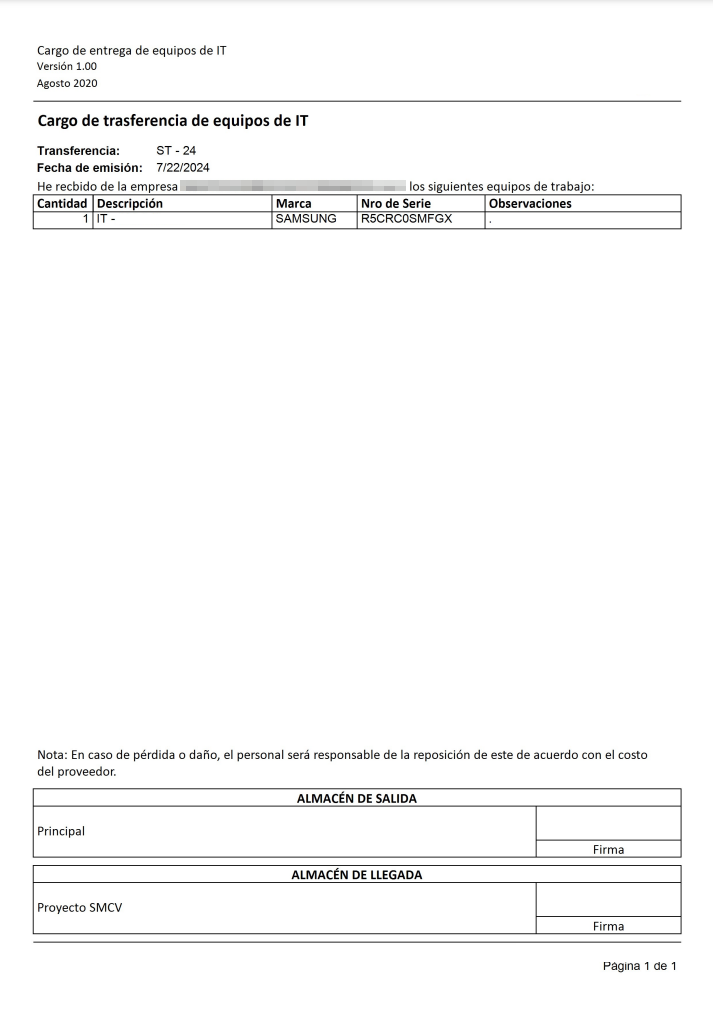
\includegraphics[width=\textwidth]{./images/reporteTransferencia.png}
    \end{subfigure}
\end{figure}

\newpage
\section{Conclusiones}
La implementaci\'on del m\'odulo de gesti\'on de inventario de equipos desarrollado para la empresa NextSoft ha cumplido con los objetivos planteados, proporcionando una soluci\'on robusta, eficiente y alineada con las necesidades operativas de la organizaci\'on. A lo largo del proyecto, se ha demostrado la importancia de una planificaci\'on meticulosa y una ejecuci\'on rigurosa, apoyada en una metodolog\'{\i}a \'agil como SCRUM, que permiti\'o un desarrollo iterativo y adaptable a los requerimientos cambiantes del entorno empresarial.
\subsection{Integraci\'on Exitosa con Sistemas Existentes}
El m\'odulo se integr\'o de manera efectiva con los sistemas existentes en la empresa, como el ERP de NextSoft, el sistema de log\'{\i}stica, el sistema de activos y el sistema de tesorer\'{\i}a. Estas integraciones no solo han optimizado los procesos de gesti\'on de inventario, evitando la duplicaci\'on de datos y automatizando tareas, sino que tambi\'en han mejorado la calidad y precisi\'on de la informaci\'on disponible para la toma de decisiones estrat\'egicas.
\subsection{Arquitectura T\'ecnica Solida}
El dise\~{n}o y la implementaci\'on del m\'odulo se realizaron utilizando tecnolog\'{\i}as modernas y probadas, como Angular 12 para el frontend y .NET 8 para el backend. La arquitectura multicapa implementada, que incluye la capa de presentaci\'on, la capa de l\'ogica de negocio, la capa de acceso a datos y la capa de servicios, ha garantizado una clara separaci\'on de responsabilidades, facilitando el mantenimiento y la escalabilidad del sistema. Adem\'as, el uso de procedimientos almacenados en SQL Server ha optimizado las operaciones de base de datos, garantizando una gesti\'on eficiente de los datos.
\subsection{Funcionalidades Clave y Experiencia de Usuario}
El m\'odulo ha proporcionado una amplia gama de funcionalidades esenciales para la gesti\'on de inventario de equipos, incluyendo el registro individual y masivo de equipos, la gesti\'on de movimientos como entregas, devoluciones y transferencias, y la generaci\'on de reportes detallados. La interfaz de usuario, dise\~{n}ada con un enfoque en la usabilidad y la eficiencia, ha permitido a los usuarios interactuar con el sistema de manera intuitiva y productiva, asegurando una curva de aprendizaje m\'{\i}nima.
\subsection{Pruebas Exhaustivas y Aseguramiento de Calidad}
Las pruebas exhaustivas realizadas durante el desarrollo, utilizando herramientas como Postman para el backend y pruebas en formularios reactivos para el frontend, han asegurado un alto nivel de calidad en el sistema. La integraci\'on entre frontend y backend fue rigurosamente probada, as\'{\i} como las operaciones de guardado y recuperaci\'on de datos desde la base de datos, garantizando que el sistema funcione de manera correcta y confiable en producci\'on.
\subsection{Resultados y Beneficios}
El m\'odulo ha resultado en una significativa mejora en la gesti\'on de inventario de equipos dentro de NextSoft. La capacidad de generar reportes detallados y espec\'{\i}ficos para cada tipo de movimiento (como cargos de entrega, devoluci\'on y transferencia) ha proporcionado a la empresa una herramienta poderosa para el seguimiento y la auditor\'{\i}a de sus activos. En resumen, este proyecto ha demostrado ser un paso fundamental hacia la modernizaci\'on y optimizaci\'on de los procesos de gesti\'on de inventario de la empresa, aline\'andose con las mejores pr\'acticas de la industria y cumpliendo con los m\'as altos est\'andares de calidad.
\subsection{Futuras Mejoras y Extensibilidad}
Finalmente, la arquitectura del sistema y su integraci\'on con los sistemas existentes en NextSoft permiten futuras mejoras y extensiones. Esto asegura que el m\'odulo puede adaptarse a las necesidades cambiantes de la empresa, soportar nuevos requerimientos y seguir aportando valor a largo plazo.
\newpage
\section{Recomendaciones}
A partir de la experiencia obtenida durante el desarrollo e implementaci\'on del m\'odulo de gesti\'on de inventario de equipos para NextSoft, se presentan las siguientes recomendaciones para maximizar el aprovechamiento del sistema y facilitar futuras mejoras:
\subsection{Capacitaci\'on Continua de los Usuarios}
Aunque el sistema fue dise\~{n}ado con un enfoque en la usabilidad y eficiencia, es recomendable realizar capacitaciones peri\'odicas para los usuarios. Esto garantizar\'a que todos los actores involucrados comprendan completamente las funcionalidades del sistema, especialmente en lo que respecta a la generaci\'on de reportes y la gesti\'on de movimientos. La familiarizaci\'on con el sistema permitir\'a a los usuarios aprovechar al m\'aximo todas sus capacidades.
\subsection{Monitoreo y Mantenimiento Regular del Sistema}
Para asegurar el correcto funcionamiento del m\'odulo a largo plazo, se recomienda establecer un plan de monitoreo y mantenimiento regular. Esto incluye la supervisi\'on del rendimiento del sistema, la actualizaci\'on de las tecnolog\'{\i}as utilizadas (como Angular y~.NET) y la optimizaci\'on de la base de datos mediante la revisi\'on peri\'odica de los procedimientos almacenados.
\subsection{Extensi\'on de Funcionalidades}
Dado que el sistema ha sido dise\~{n}ado con una arquitectura modular y escalable, se recomienda evaluar la posibilidad de extender las funcionalidades del m\'odulo en futuras fases. Por ejemplo, podr\'{\i}a incorporarse un sistema de notificaciones automatizadas para alertar a los usuarios sobre eventos clave, como el vencimiento de mantenimientos o la necesidad de reabastecer inventarios espec\'{\i}ficos.
\subsection{Mejora en la Integraci\'on con Otros Sistemas}
Aunque la integraci\'on actual con el ERP de NextSoft, el sistema de log\'{\i}stica, el sistema de activos y el sistema de tesorer\'{\i}a ha sido exitosa, se recomienda explorar opciones para una integraci\'on m\'as profunda. Por ejemplo, automatizar la actualizaci\'on de inventarios en tiempo real o integrar el sistema con herramientas de an\'alisis de datos podr\'{\i}a proporcionar a la empresa una visi\'on a\'un m\'as completa y din\'amica de su gesti\'on de equipos.
\subsection{Revisi\'on Peri\'odica de la Seguridad del Sistema}
La seguridad es un aspecto cr\'{\i}tico, especialmente cuando el sistema maneja informaci\'on sensible. Se recomienda realizar auditor\'{\i}as de seguridad peri\'odicas para identificar y mitigar posibles vulnerabilidades. Esto incluye la revisi\'on de las pol\'{\i}ticas de autenticaci\'on, la protecci\'on de los datos en tr\'ansito y en reposo, y la implementaci\'on de mecanismos de control de acceso m\'as detallados si fuera necesario.
\subsection{Evaluaci\'on de la Satisfacci\'on del Usuario}
Para asegurar que el sistema sigue cumpliendo con las expectativas y necesidades de los usuarios, es recomendable realizar encuestas de satisfacci\'on peri\'odicas. Esto permitir\'a identificar \'areas de mejora y ajustar el sistema en funci\'on de las experiencias y sugerencias de los usuarios finales.
\subsection{Documentaci\'on y Actualizaci\'on Constante}
Es fundamental mantener una documentaci\'on actualizada y accesible para todos los desarrolladores y usuarios del sistema. Esto incluye manuales de usuario, gu\'{\i}as t\'ecnicas y documentaci\'on sobre la arquitectura del sistema. Mantener esta documentaci\'on al d\'{\i}a facilitar\'a el mantenimiento futuro del sistema y asegurar\'a la continuidad del conocimiento, incluso si el equipo de desarrollo cambia.
\subsection{Exploraci\'on de Nuevas Tecnolog\'{\i}as}
Finalmente, se recomienda estar atentos a la evoluci\'on de las tecnolog\'{\i}as utilizadas en el proyecto. La r\'apida evoluci\'on de frameworks como Angular y plataformas como~.NET podr\'{\i}a ofrecer nuevas herramientas y enfoques para mejorar el rendimiento, la seguridad y la usabilidad del sistema en el futuro. Evaluar estas tecnolog\'{\i}as y planificar actualizaciones puede ser clave para mantener el sistema a la vanguardia.

Siguiendo estas recomendaciones, NextSoft puede asegurarse de que el m\'odulo de gesti\'on de inventario de equipos siga siendo una herramienta valiosa, eficaz y alineada con los objetivos estrat\'egicos de la empresa, garantizando su relevancia y eficiencia a largo plazo.
\newpage
\bibliography{bibliography}
\nocite{*}
\end{document}
